%\documentclass[10pt]{beamer}
\documentclass[xcolor={pdftex,dvipsnames,table}]{beamer}

\definecolor{redUnipd}{HTML}{9b0014}
\definecolor{grayUnipd}{HTML}{444F51}
\definecolor{myblue}{HTML}{317a9b}
%\definecolor{Black}{RGB}{0,62,114}
\newcommand{\bbf}[1]{\textcolor{black}{\bf #1}}
\newcommand{\rbf}[1]{\textcolor{redUnipd}{ #1}}
\usefonttheme{structurebold}
\usecolortheme[named=myblue]{structure}
\setbeamercolor{structure}{fg=redUnipd}
\setbeamercolor{normal text}{bg=white,fg=grayUnipd}
\setbeamertemplate{itemize items}{$\circ$}
%\textopenbullet
%\usepackage{marvosym}
%\setbeamertemplate{itemize items}{$\Neutral$}

\usepackage{pgfpages}
\pgfpagesuselayout{resize to}[a4paper, 
                                border shrink=1.5cm,
                                landscape]


\usepackage[T1]{fontenc}
%
\usepackage[english]{babel}
\usepackage{graphicx}
\usepackage{booktabs}
\usepackage{latexsym}
\usepackage{subfigure}
\usefonttheme{professionalfonts}
%\usepackage{enumitem}
\usepackage{amsmath,amssymb}
\usepackage[latin1]{inputenc}
%\setbeamercovered{dynamic}
\usepackage{Sweave}
\usepackage[english]{babel}
\usepackage{tikz,comment,amssymb}
\usetikzlibrary{shapes}

\newcommand{\bb}[1]{\begin{block}{#1}}
\newcommand{\eb}{\end{block}}
\newcommand{\bi}{\begin {itemize}}
\newcommand{\ei}{\end{itemize}}
\newcommand{\be}{\begin {enumerate}}
\newcommand{\ee}{\end{enumerate}}
\linespread{1.05}

\newcommand{\bfr}[1]{\begin{frame} \frametitle{#1}}

\AtBeginSection[] {
  \begin{frame}<beamer>
    \frametitle{Outline}
    \tableofcontents[currentsection]
  \end{frame}
}

\newcommand{\gbf}[1]{\textcolor{grayUnipd}{#1}}
\newcommand{\redUnipd}[1]{\textcolor{redUnipd}{#1}}
\newcommand{\grayUnipd}[1]{\textcolor{grayUnipd}{#1}}

\newcommand{\XX}{\mathbf{X}}
\newcommand{\YY}{\mathbf{Y}}
\newcommand{\yy}{\mathbf{y}}
\newcommand{\xx}{\mathbf{x}}
\newcommand{\ZZ}{\mathbf{Z}}
\newcommand{\WW}{\mathbf{W}}
\newcommand{\Orbit}{\mathcal{O}}
\newcommand{\II}{\mathbf{I}}
\newcommand{\flip}{\mathbf{g}}
\newcommand{\nnu}{\nu}
\newcommand{\ones}{\mathbf{1}}
\newcommand{\Ifisher}{\mathcal{I}}
\newcommand{\norm}{||}
\newcommand{\simDot}{\overset{.}{\sim}}

\AtBeginSection[] {
  \begin{frame}<beamer>
    \frametitle{Outline}
    \tableofcontents[currentsection]
 \end{frame}
}


\title{Permutation tests for Clinical Trials}
\author{Livio Finos}
\date{}%17/02/16}
% \logo{
\includegraphics[scale=.1]{figures/logoUnipd.jpg}}

\begin{document}
\begin{frame}
\titlepage
\end{frame}

%% ==========================TITLE PAGE
\section{Introduction}

\bfr{Introduction}
\bi
\item Well established nonparametric approach to {\bf inference}: Fisher, 1935; Pitman, 1937; Pitman, 1938. 
\item (In general) it requires less assumptions about the data generating process than the parametric counterpart. 
\item Very good inferential properties, typically:
 \bi 
 \item exactness (i.e. exact control of the type I error)
 \item asymptotically optimality and convergence to the parametric counterpart when it does exist.
\ei
\ei

\end{frame}
\bfr{Introduction}
\bi
\item Fisher exact test is a prototypical example, but
\item  the general approach has restricted applicability without the support of a computer. %This is the case of very small datasets where all possible rearrangement of the data can be enumerated. In all other cases, only special cases can be treated ’by hand’. The most well-known example is the comparison of two independent samples with a binomial response, that is, the 
\ei
\end{frame}
\bfr{Renewed interest toward permutation testing}
\bi
\item A milestone: Westfall and Young (1993). Resampling-Based Multiple Testing: 
Examples and Methods for p-value Adjustment. Wiley.
\item Many actives areas of research adopt these methods in their daily statistical analysis (e.g. genetics and neuroscience: Nichols and Holmes (2002); Pantazis et al. (2009); Winkler et al. (2014)).
\item Permutation approach:
\bi 
\item Ideal for {\bf randomized experimental design}
\item deals with very complex
models,  without formal definition of the data generating process.
\ei
\ei

\end{frame}

%%%%%%%%%%%%%%%%%
% \section{Conditional (permutations) testing}
% \bfr{Renaissance of permutation tests}
% Computationally intensive, but usually
% \bi
% \item require less assumptions
% \item exact control of Type I Error, also for small sample size
% \item converge to parametric counterpart \\ (ie asymptotically same power)
% \item multivariate (multiplicity correction): easy and powerful 
% \ei
% \end{frame}
%%%%%%%%%%%%%%%%%
%%%%%%%%%%%%%%%%%%%%%%%%%%%%%%%
%%%%%%%%%%%%%%%%%%%%%%%%%%%%%%%%
%%%%%%%%%%%%%%%%%%%%%%%%%%%%%%%%
\section{A toy example} 
\begin{frame}{A Naive approach to Permutation Testing}
\bb{Comparison of Two Samples (i.e. one factor with two levels)} 
\bi 
\item[$\cdot$] {\bf Control}: 3 observations,
\item[$\cdot$] \rbf{Treated}: 3 observations:
\ei
$$\gbf{1.025}, \gbf{1.949}, \gbf{3.477}, \rbf{2.391}, \rbf{3.676}, \rbf{4.816}$$
\eb
\bb{Hypothesis testing} 
\bi 
\item $H_0$: Two groups are equal
\item $H_1$: Treated is greater than Control (on average)
\ei
\eb
\rbf{$p$-value}: probability to get the observed evidence against $H_0$ if the two groups were equal (i.e.  $H_0$ were true)\\
\rbf{Test}: if $p\leq\alpha$ (e.g. $\alpha=.05$): we decide for $H_1$,\\\qquad\ \  otherwise: we stay with $H_0$ 
\end{frame}
%%%%%%%%%%%%%%%%%%
\bfr{Parametric approach}
Assumptions on $y_1,y_2,\ldots,y_6$
\bi
\item independent
\item identically distributed
\item[] \bi
  \item normally distributed% $N(\mu_{Treated},\sigma^2)$ and $N(\mu_{Control},\sigma^2)$
  \item[] OR
  \item have finite mean and variance (but inference is only asymptotically valid in this case!)
  \ei
\ei
\pause

We can perform a t-test:
 $$T=\frac{\bar{y}(Treated)-\bar{y}(Control)}
 {\widehat{sd(\bar{y}(Treated)-\bar{y}(Control))}}\sim t_4$$
(i.e. T test statistic follow a $t$ distribution with n-2=4 d.f.)
\end{frame}
%%%%%%%%%%%%%%%%%%
\bfr{Parametric approach}

With toy data:\\
{\tt t = -1.4545, \\
df = 4,\\
p-value = 0.1098}
\bigskip

\bb{Remark}
The hypotheses tested are:
\bi
\item $H_0: \mu_{Treated}=\mu_{Control}$
\item $H_1: \mu_{Treated}>\mu_{Control}$ (only a difference in mean is allowed)
\ei
\eb
\end{frame}
%%%%%%%%%%%%%%%%%%%%%
\section{A Naive approach to Permutation Testing}
\bfr{A Naive approach to Permutation Testing}
The $p$-value is computed \bbf{under $H_0$:} \\
\gbf{Controls} and \rbf{Treated} have the \bbf{same distribution}.
\bigskip

\bb{Collection of equally likely outcomes:}
\begin{eqnarray*}
&&f(\gbf{1.025}, \gbf{1.949}, \gbf{3.477}, \rbf{2.391}, \rbf{3.676}, \rbf{4.816}) =\\ \pause
&=&f(\gbf{1.025}, \rbf{1.949}, \gbf{3.477}, \rbf{2.391}, \gbf{3.676}, \rbf{4.816})=\\ \pause
&=&f(\rbf{1.025}, \rbf{1.949}, \gbf{3.477}, \gbf{2.391}, \rbf{3.676}, \gbf{4.816})=\\ \pause
&=& \ldots
\end{eqnarray*}
\eb

There are ${6 \choose 3}=\frac{6!}{3!3!}=20$ equally likely outcomes

\end{frame}

\bfr{A Naive approach to Permutation Testing}
Compute the difference in mean of the two samples
\begin{center}
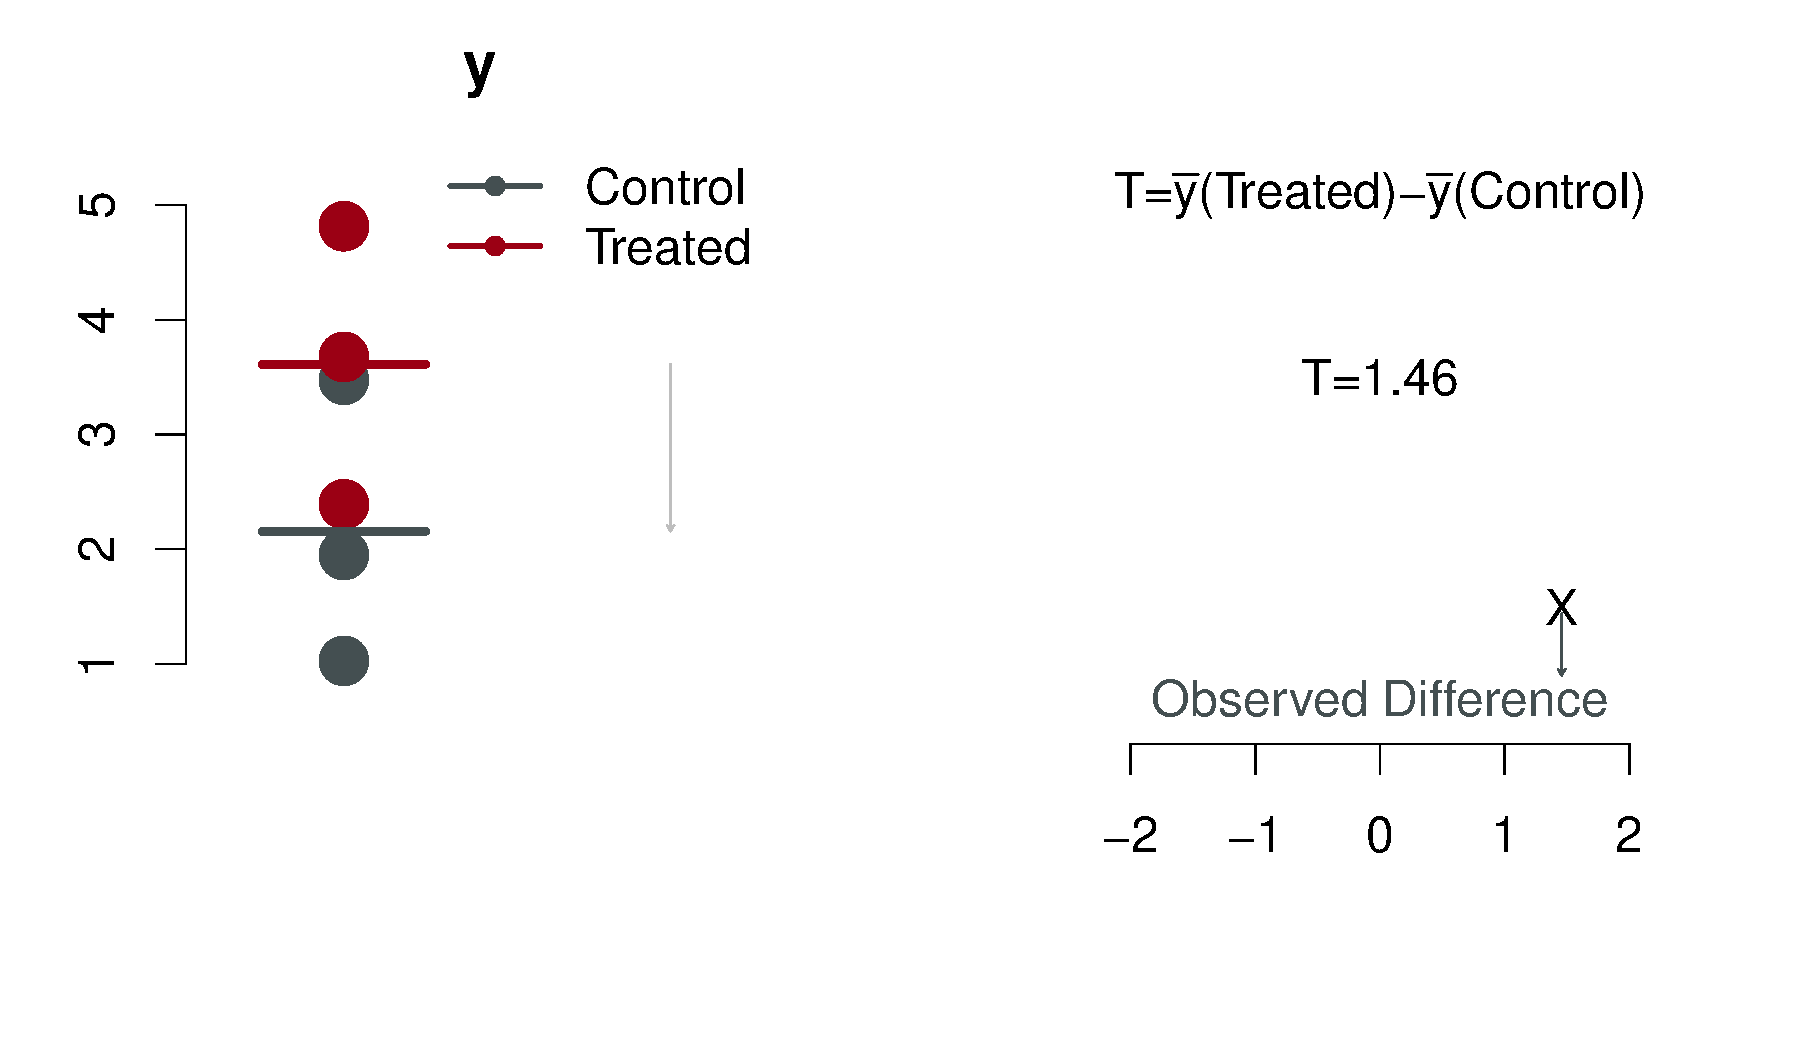
\includegraphics[width=1.1\textwidth]{figures/permsslides1} 
\end{center}
\end{frame}


\bfr{A Naive approach to Permutation Testing}
Compute the same difference on another hypothetical experiment
\begin{center}
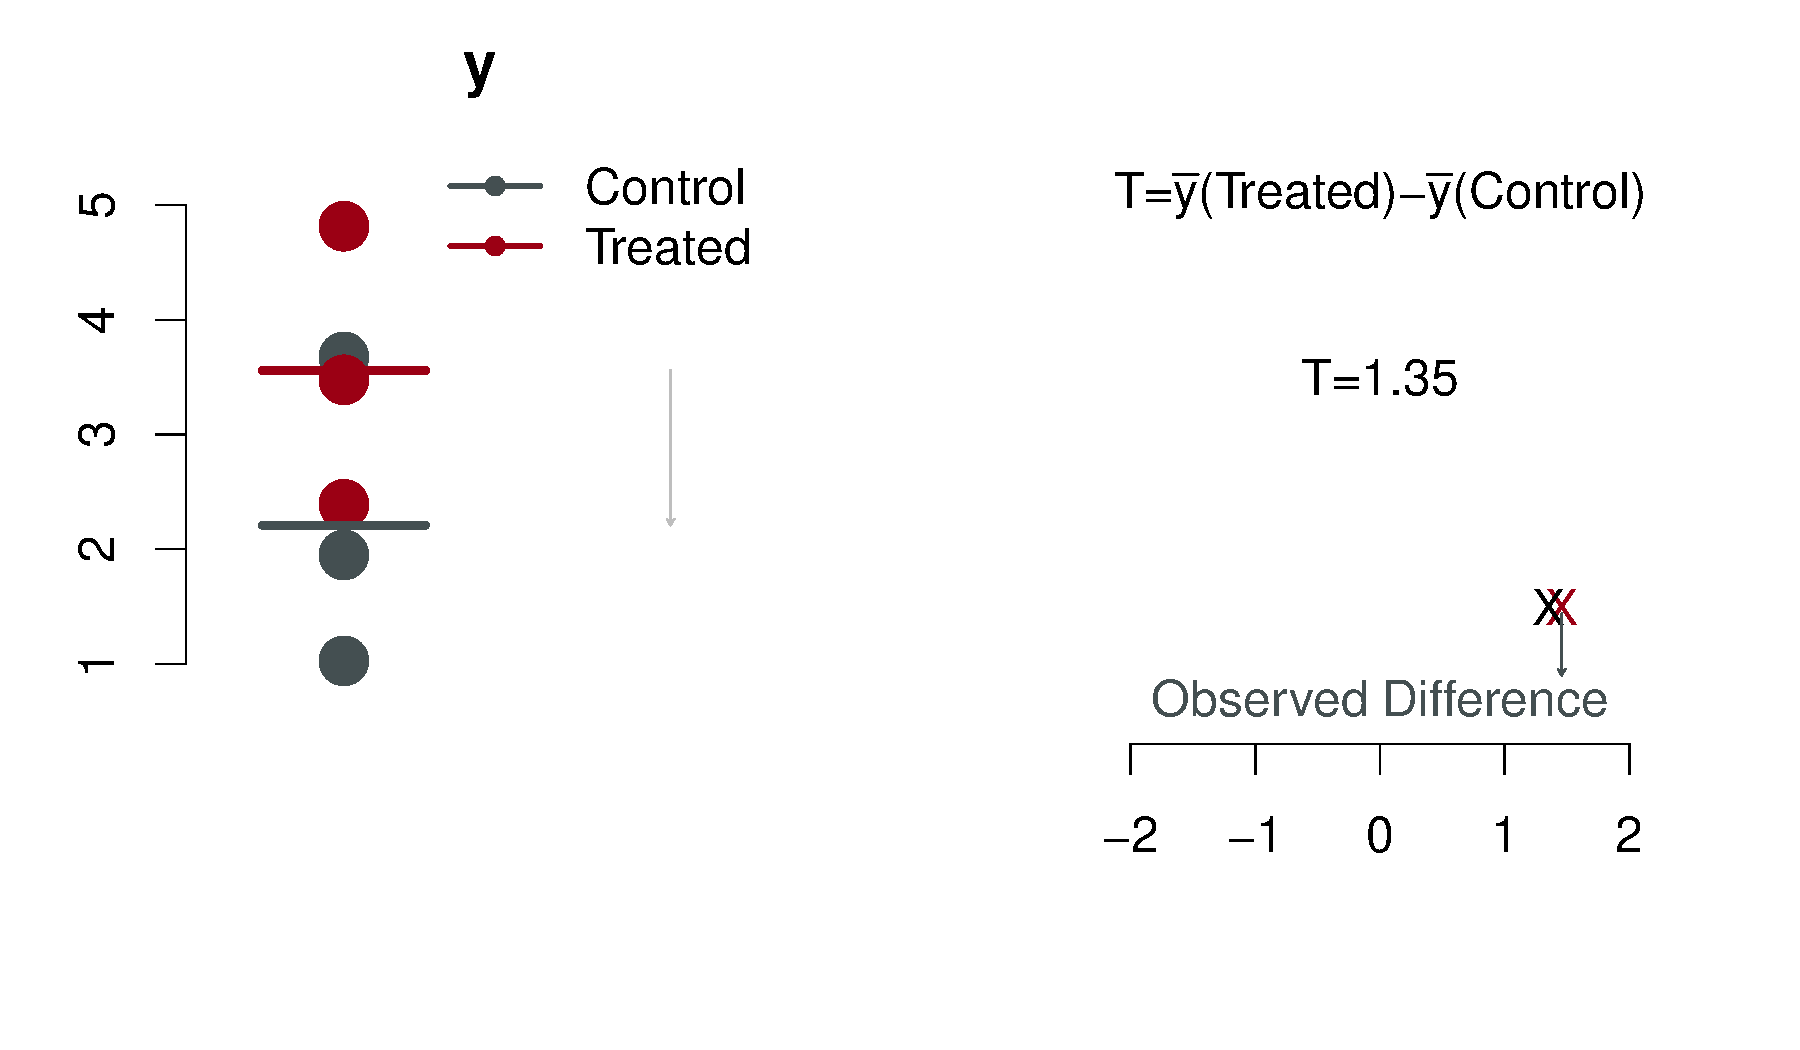
\includegraphics[width=1.1\textwidth]{figures/permsslides2} 
\end{center}
\end{frame}


\begin{frame}{A Naive approach to Permutation Testing}
\ldots and go on with all hypothetical experiments\ldots
\begin{center}
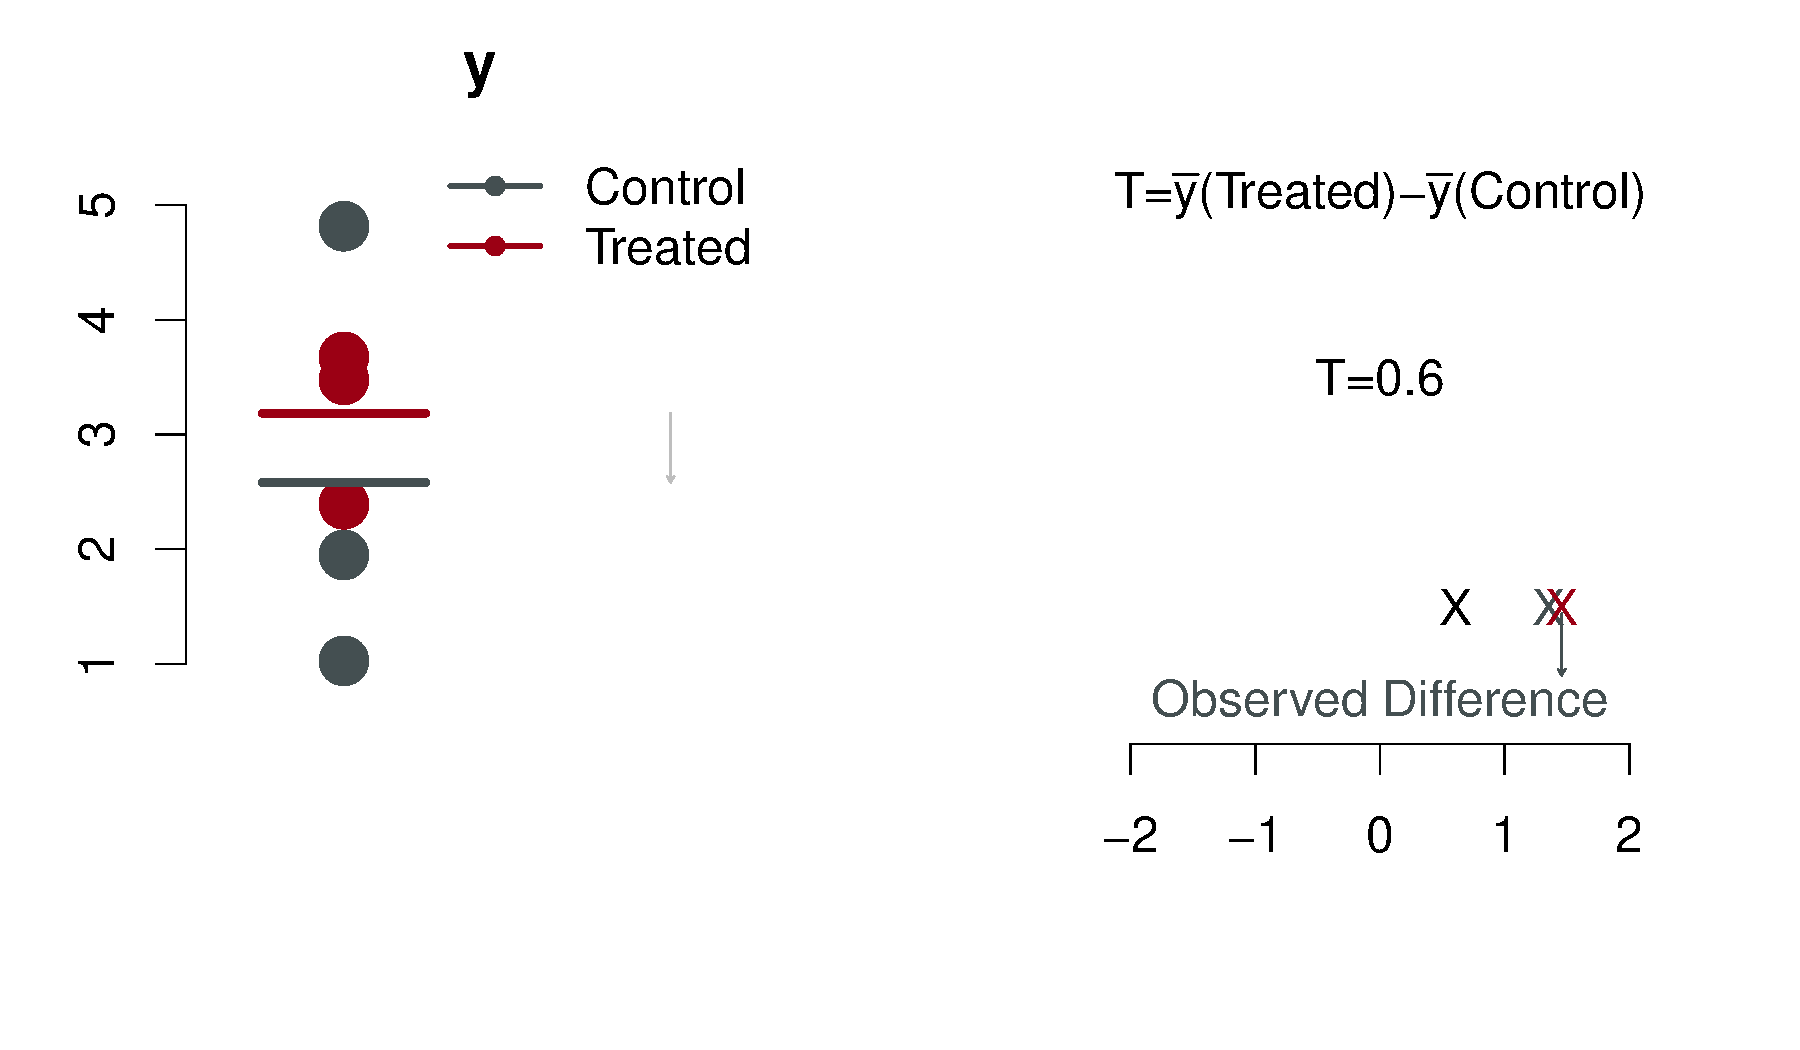
\includegraphics[width=1.1\textwidth]{figures/permsslides3} 
\end{center}
\end{frame}


\begin{frame}{A Naive approach to Permutation Testing} 
\ldots and go on with all hypothetical experiments\ldots
\begin{center}
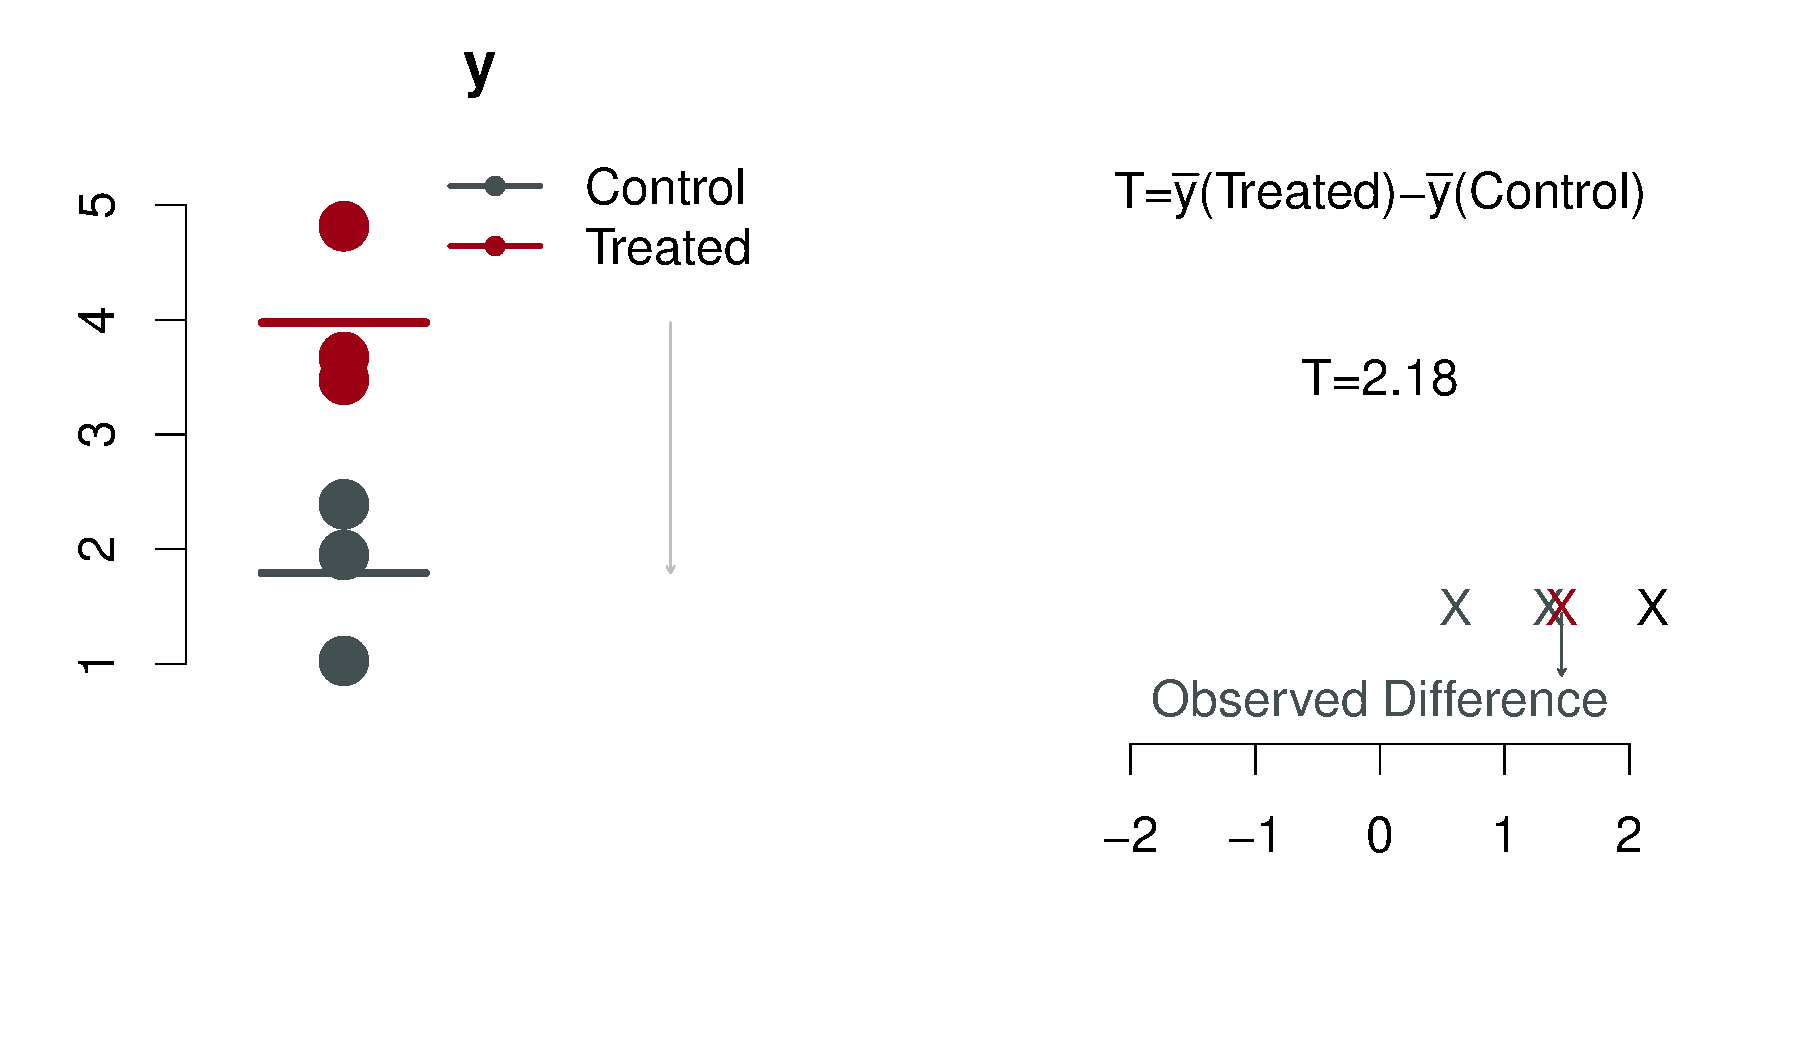
\includegraphics[width=1.1\textwidth]{figures/permsslides4} 
\end{center}
\end{frame}



\begin{frame}{A Naive approach to Permutation Testing} 
\ldots and go on with all hypothetical experiments\ldots
\begin{center}
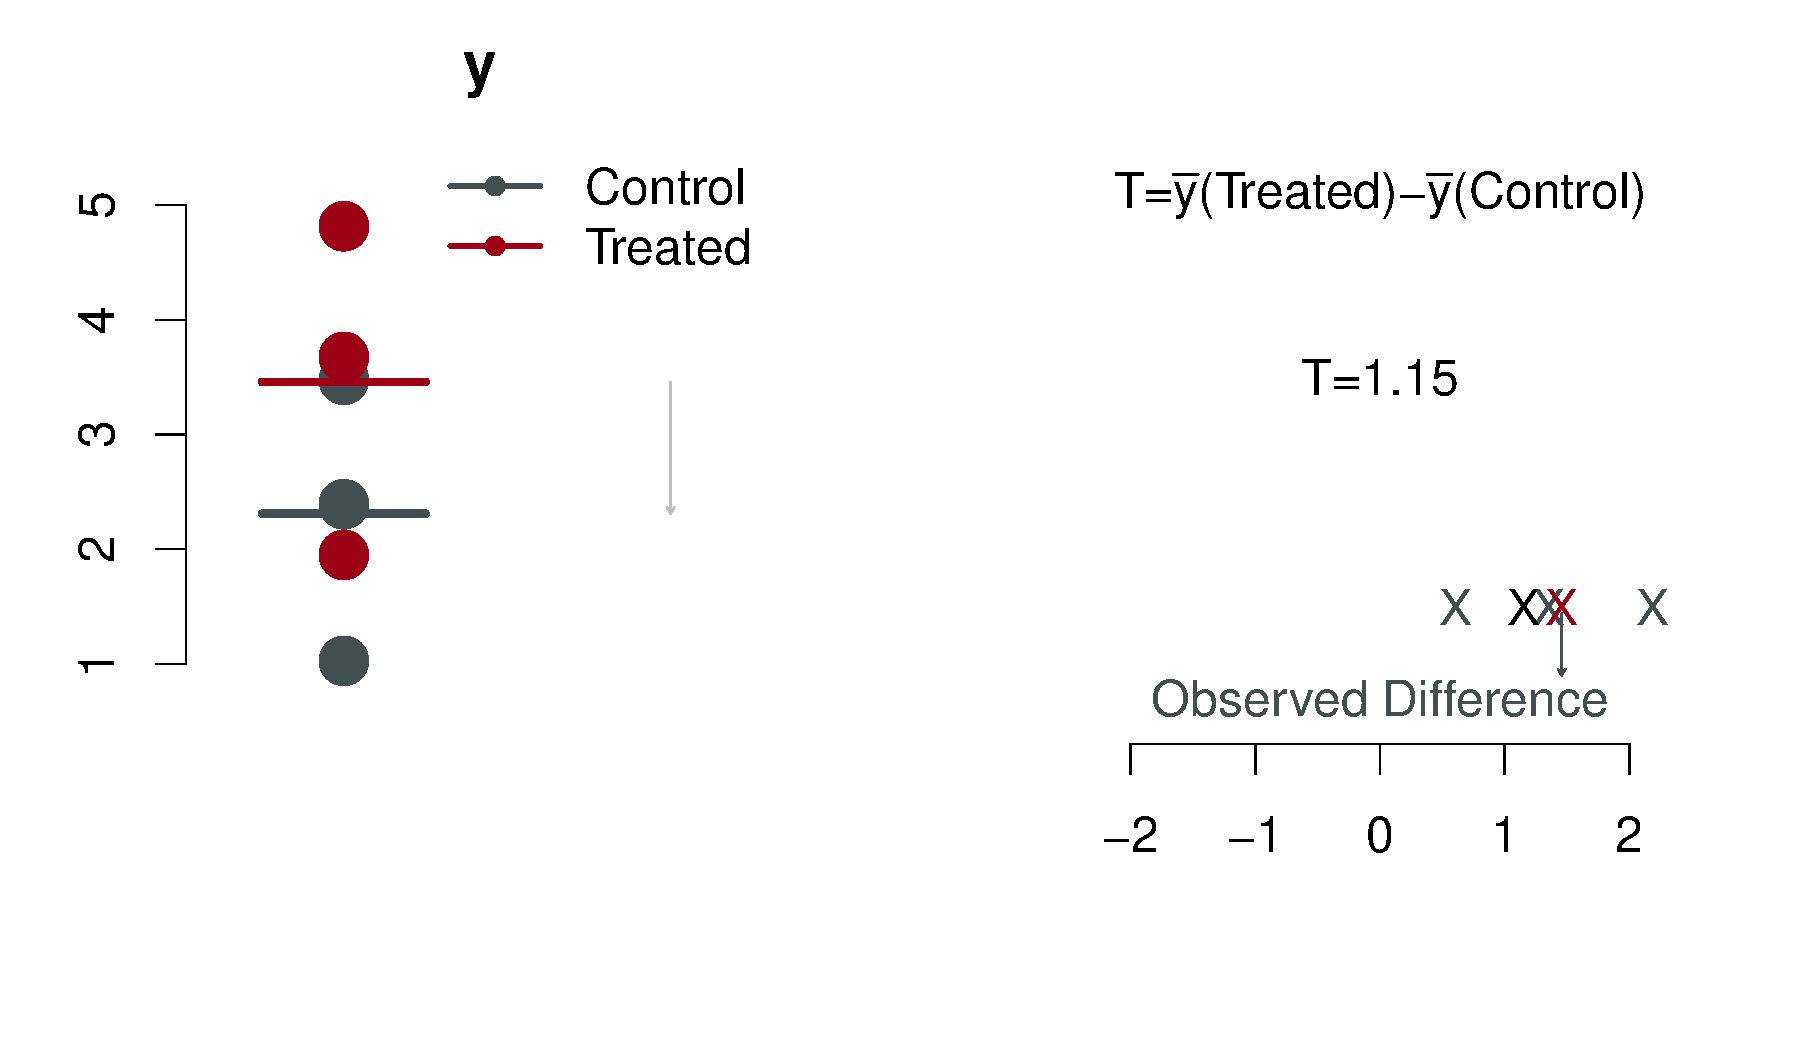
\includegraphics[width=1.1\textwidth]{figures/permsslides5} 
\end{center}
\end{frame}


\begin{frame}{A Naive approach to Permutation Testing}
\ldots and go on with all hypothetical experiments\ldots
\begin{center}
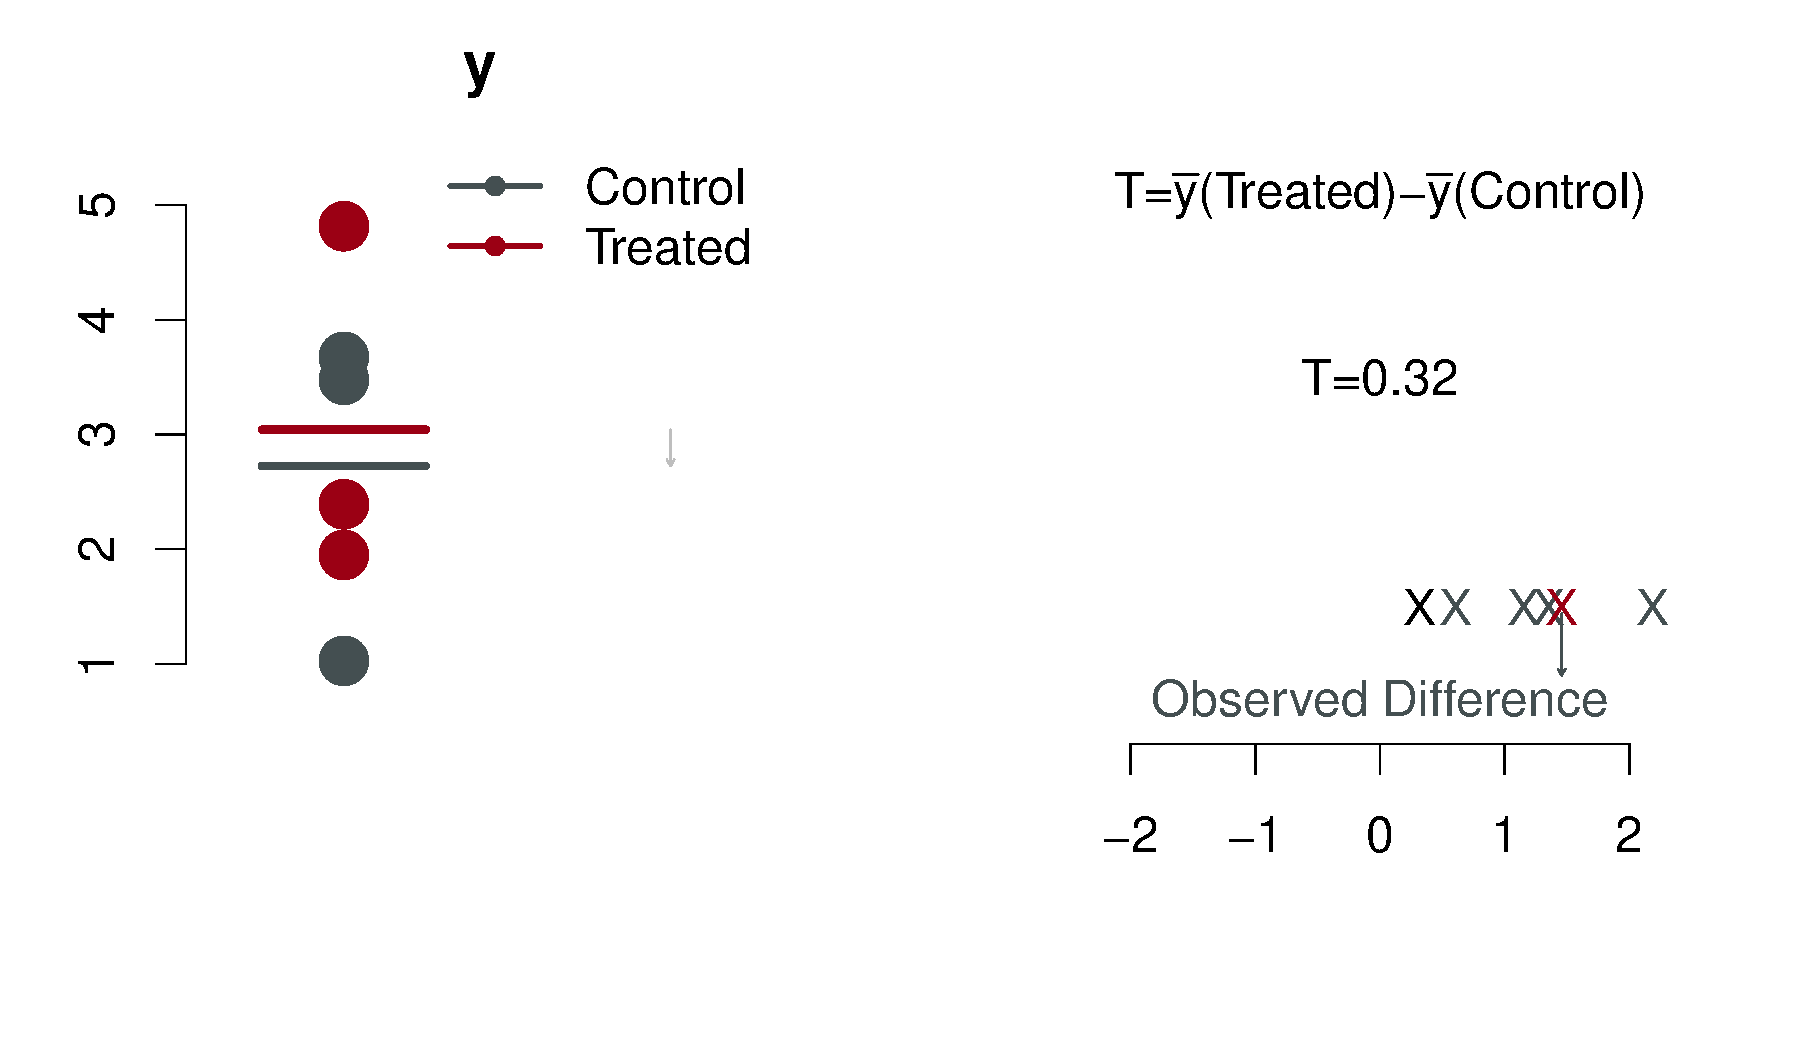
\includegraphics[width=1.1\textwidth]{figures/permsslides6} 
\end{center}
\end{frame}


\begin{frame}{A Naive approach to Permutation Testing}
\ldots and go on with all hypothetical experiments\ldots
\begin{center}
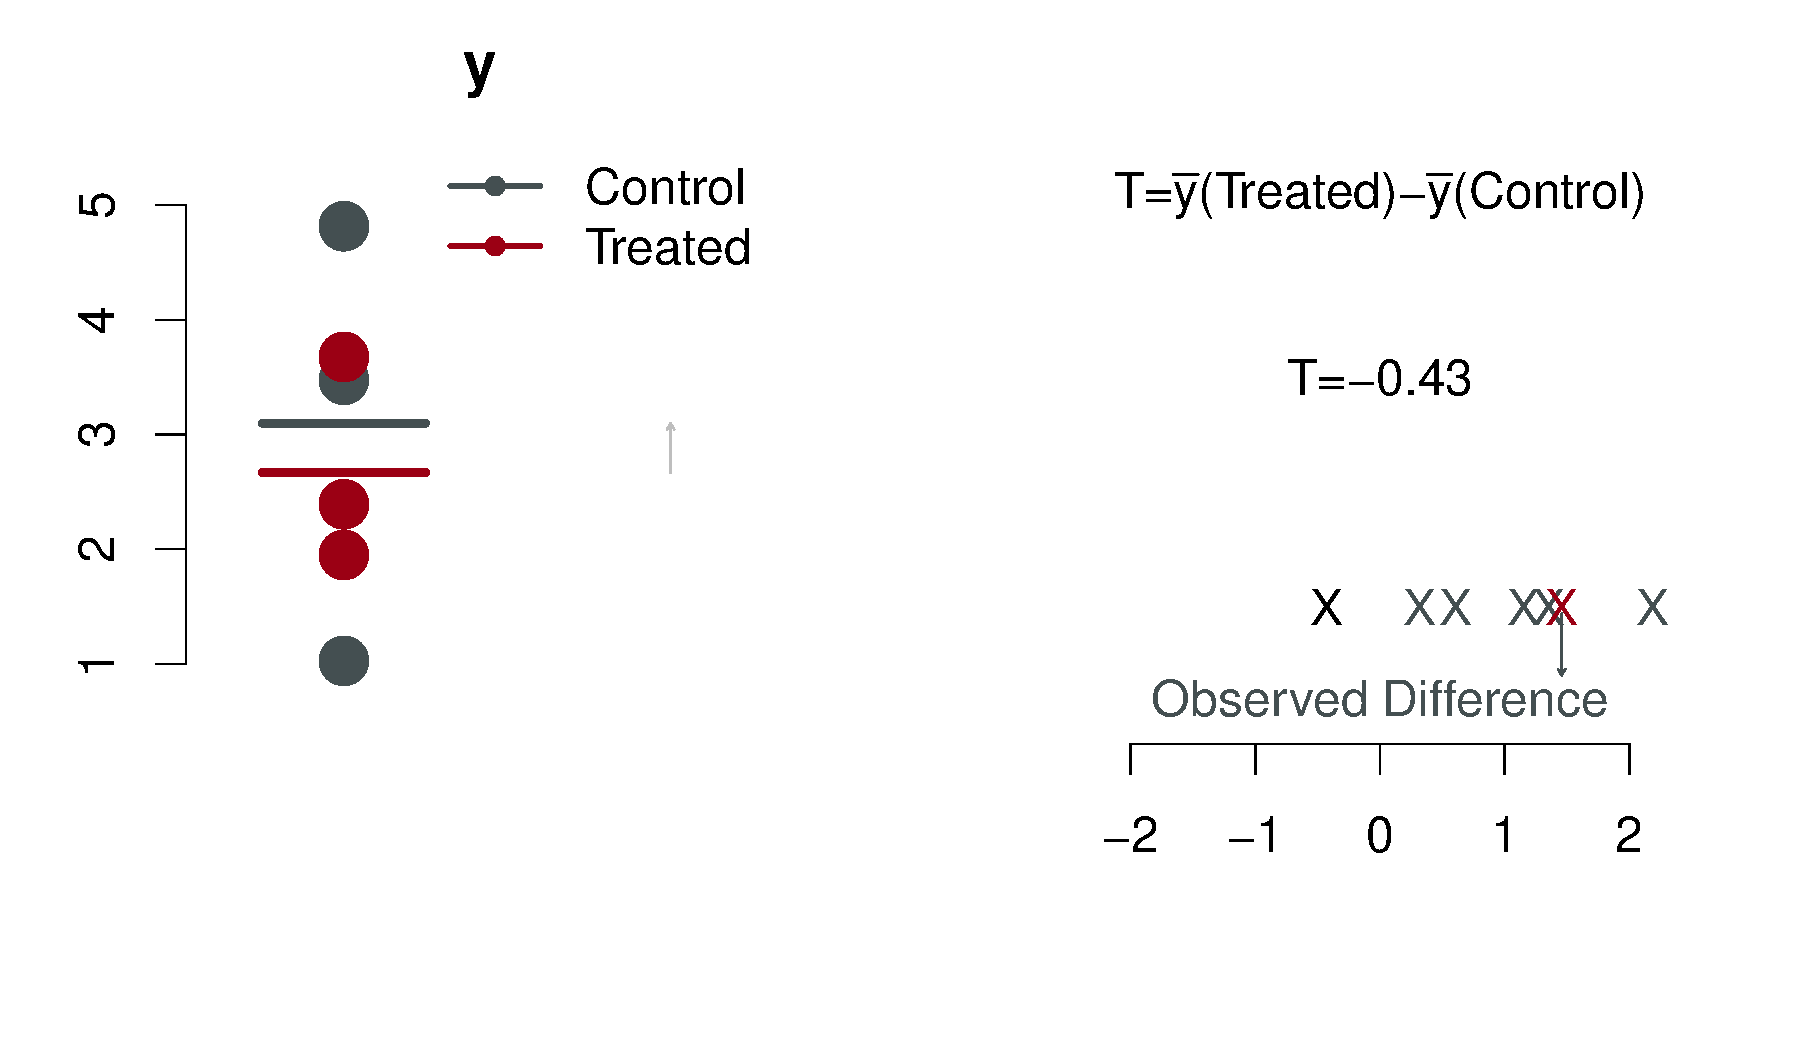
\includegraphics[width=1.1\textwidth]{figures/permsslides7} 
\end{center}
\end{frame}



\begin{frame}{A Naive approach to Permutation Testing}
\ldots and go on with all hypothetical experiments\ldots
\begin{center}
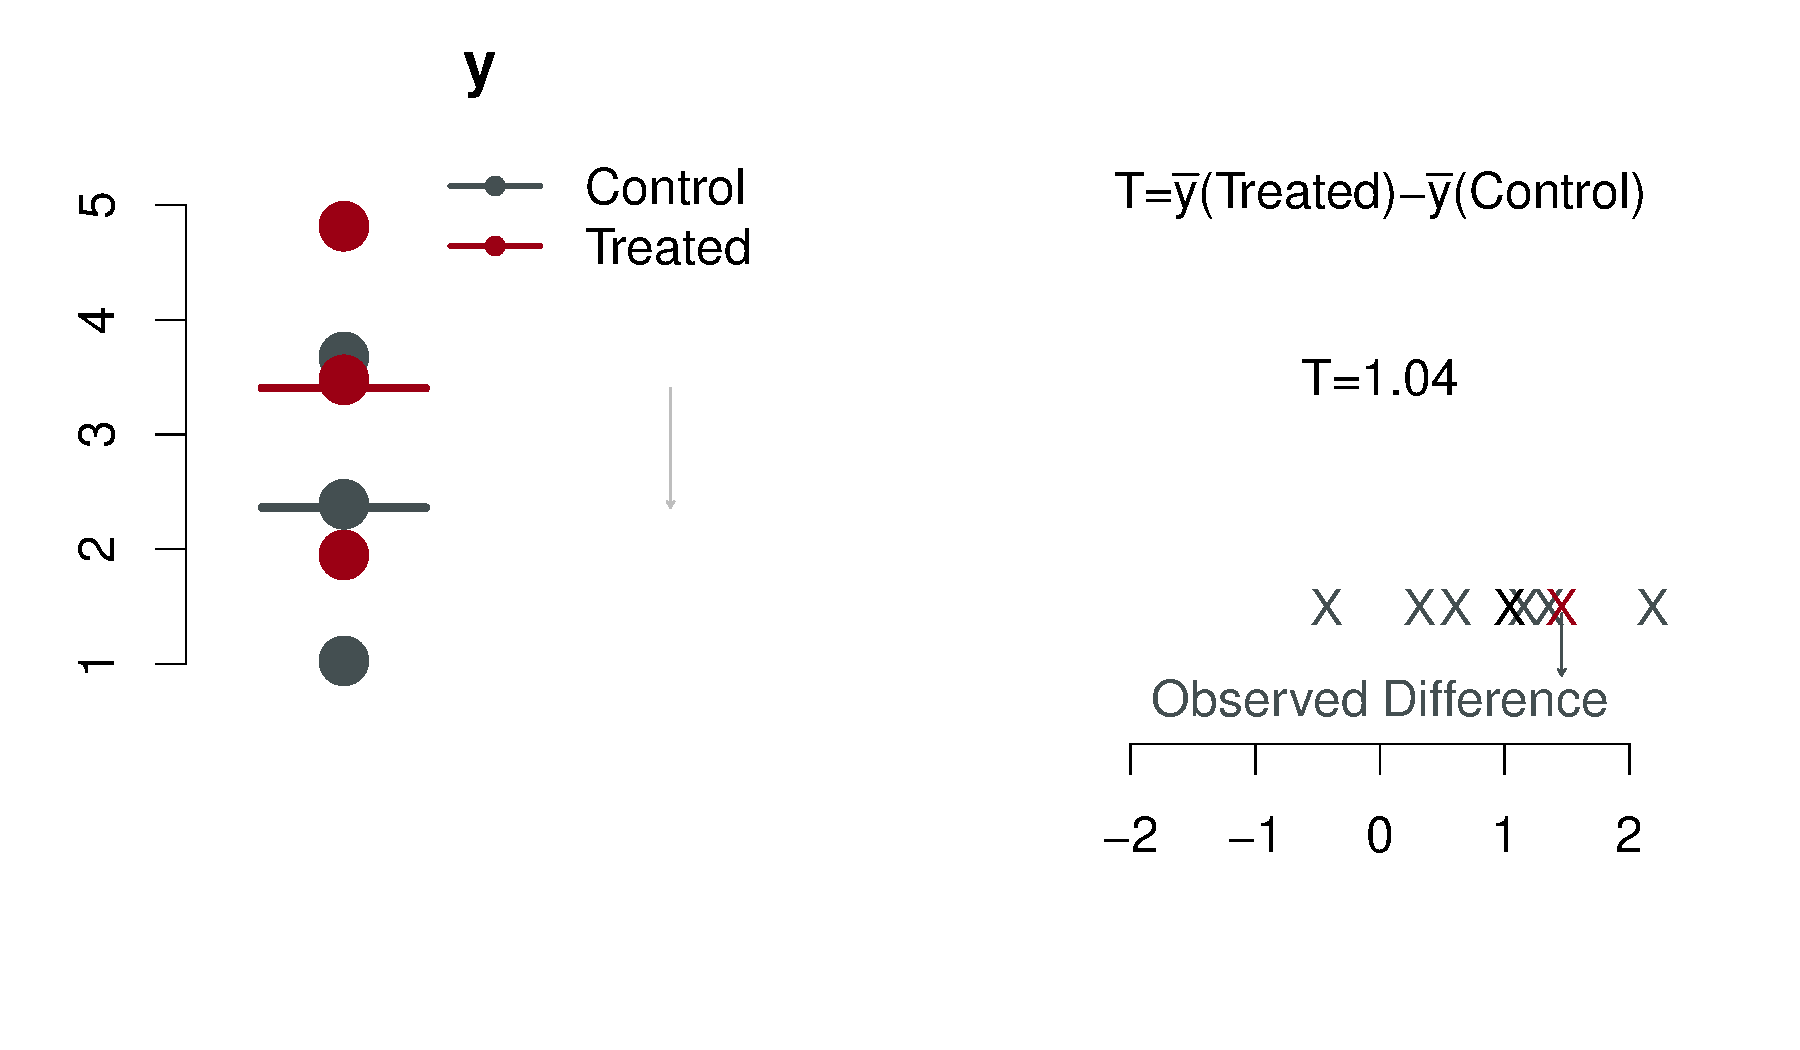
\includegraphics[width=1.1\textwidth]{figures/permsslides8} 
\end{center}
\end{frame}


\begin{frame}{A Naive approach to Permutation Testing} 
\ldots and go on with all hypothetical experiments\ldots
\begin{center}
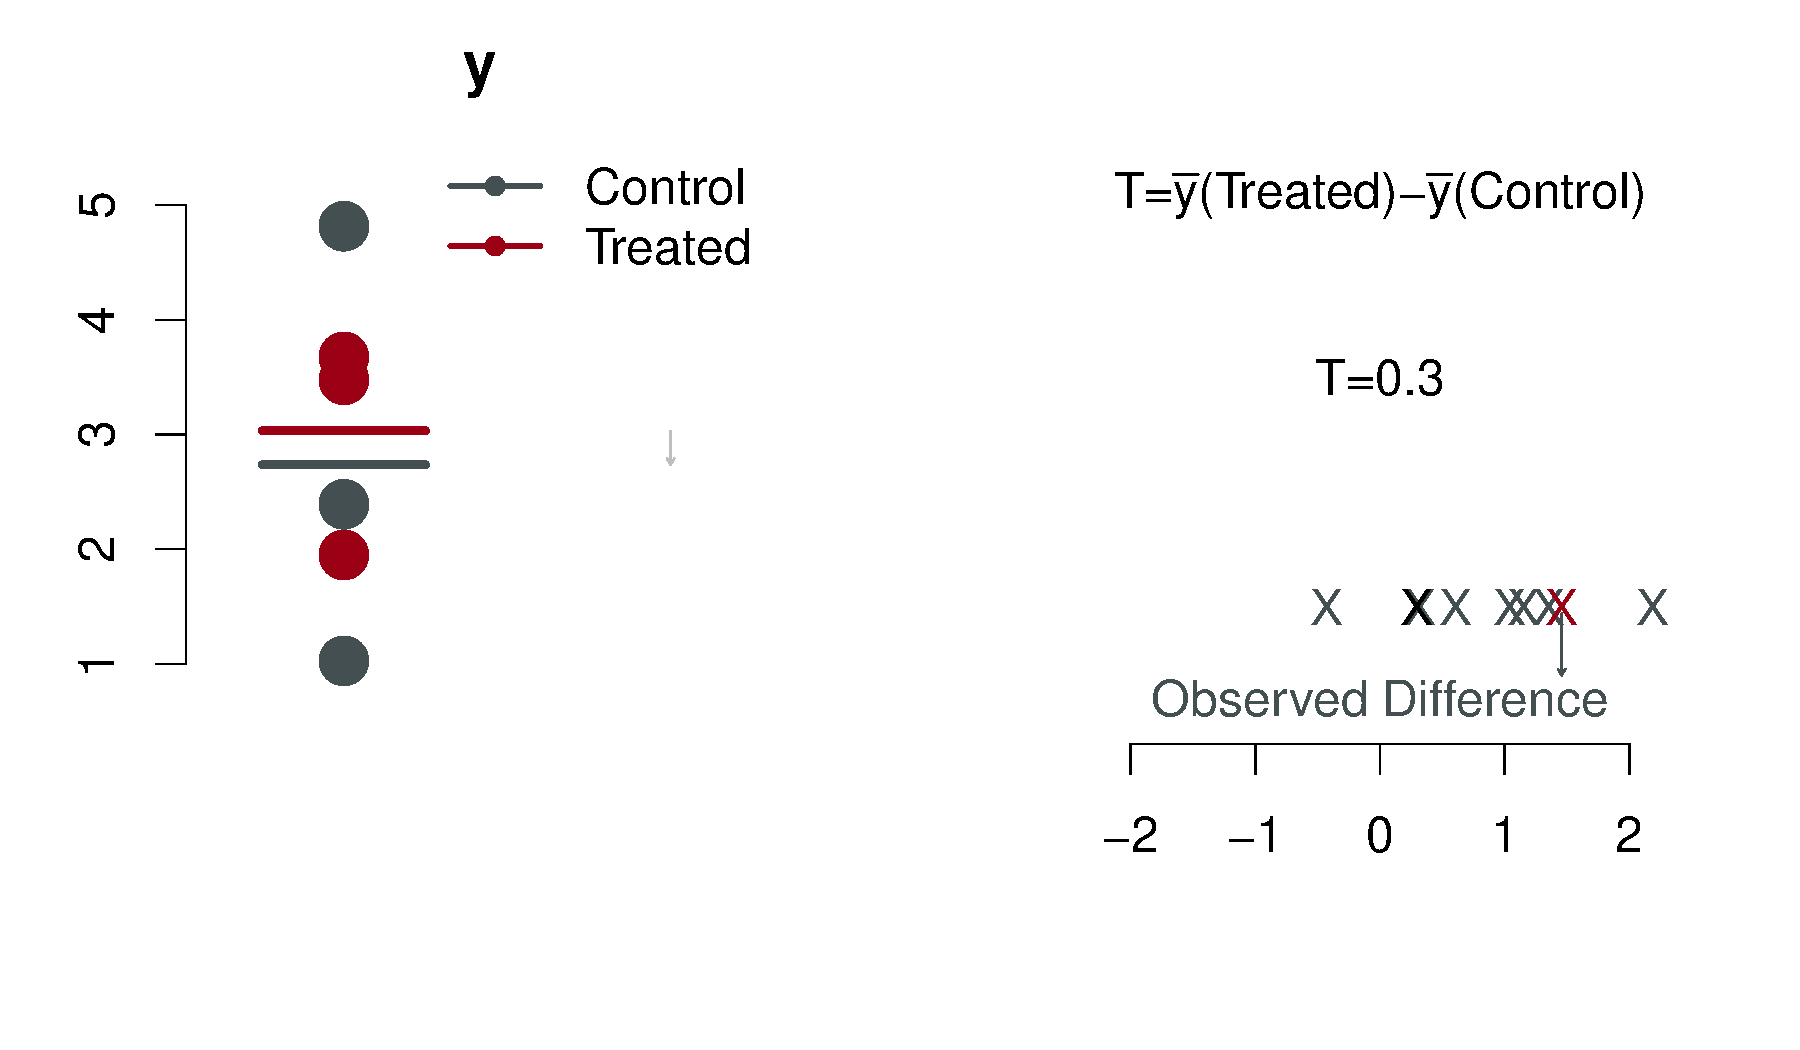
\includegraphics[width=1.1\textwidth]{figures/permsslides9} 
\end{center}
\end{frame}


\begin{frame}{A Naive approach to Permutation Testing}
\ldots and go on with all hypothetical experiments\ldots
\begin{center}
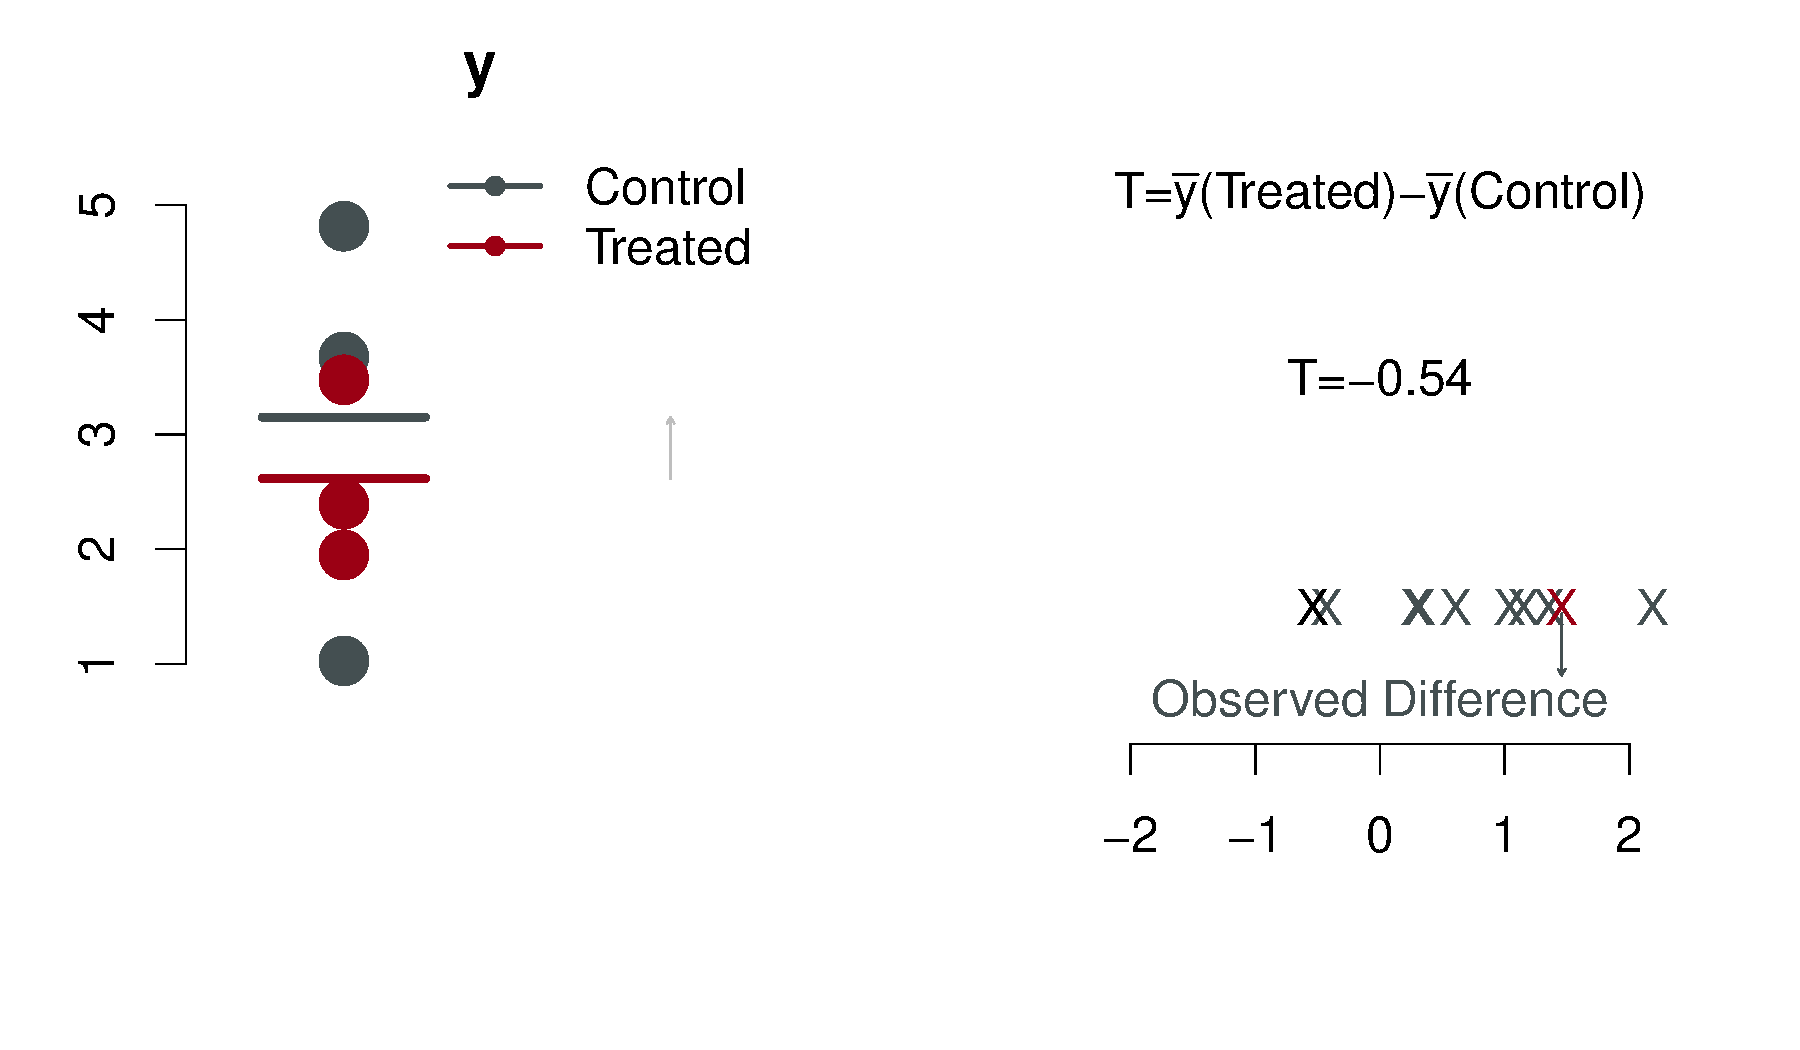
\includegraphics[width=1.1\textwidth]{figures/permsslides10} 
\end{center}
\end{frame}


\begin{frame}{A Naive approach to Permutation Testing}
 \ldots and go on with all hypothetical experiments\ldots 
\begin{center}
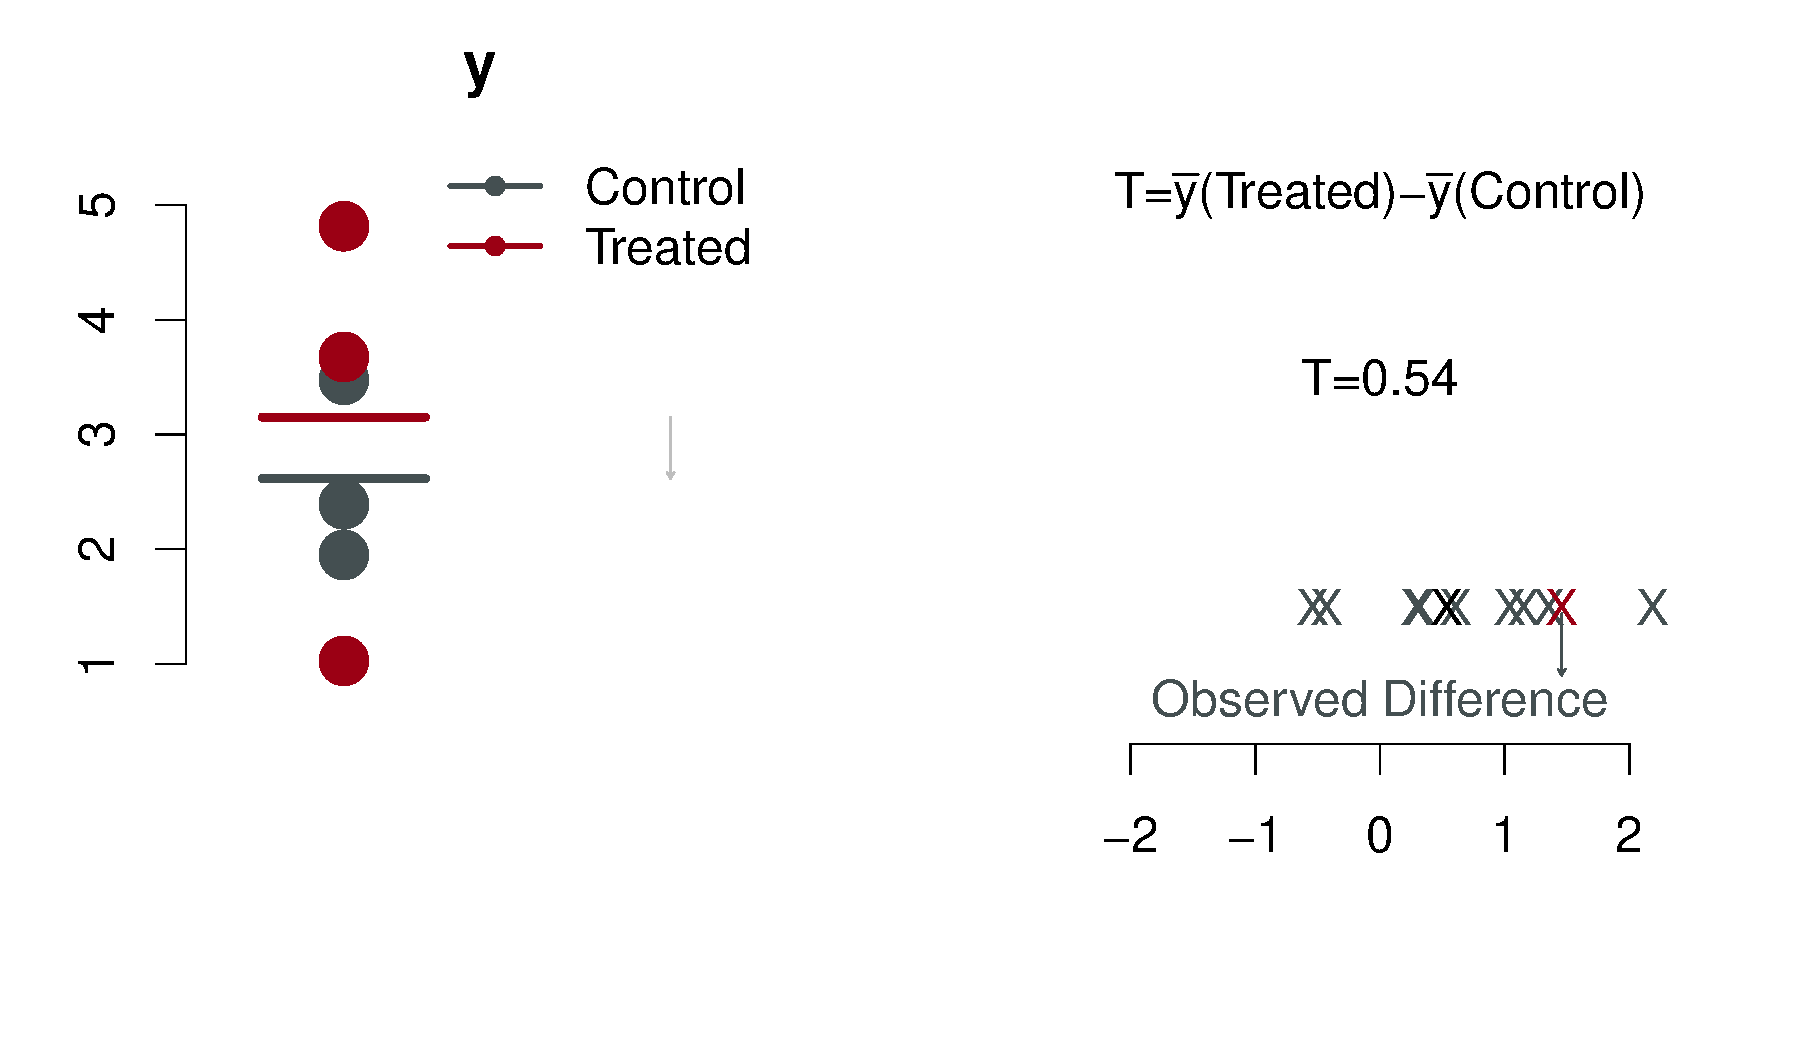
\includegraphics[width=1.1\textwidth]{figures/permsslides11} 
\end{center}
\end{frame}


\begin{frame}{A Naive approach to Permutation Testing}
 \ldots and go on with all hypothetical experiments\ldots 
\begin{center}
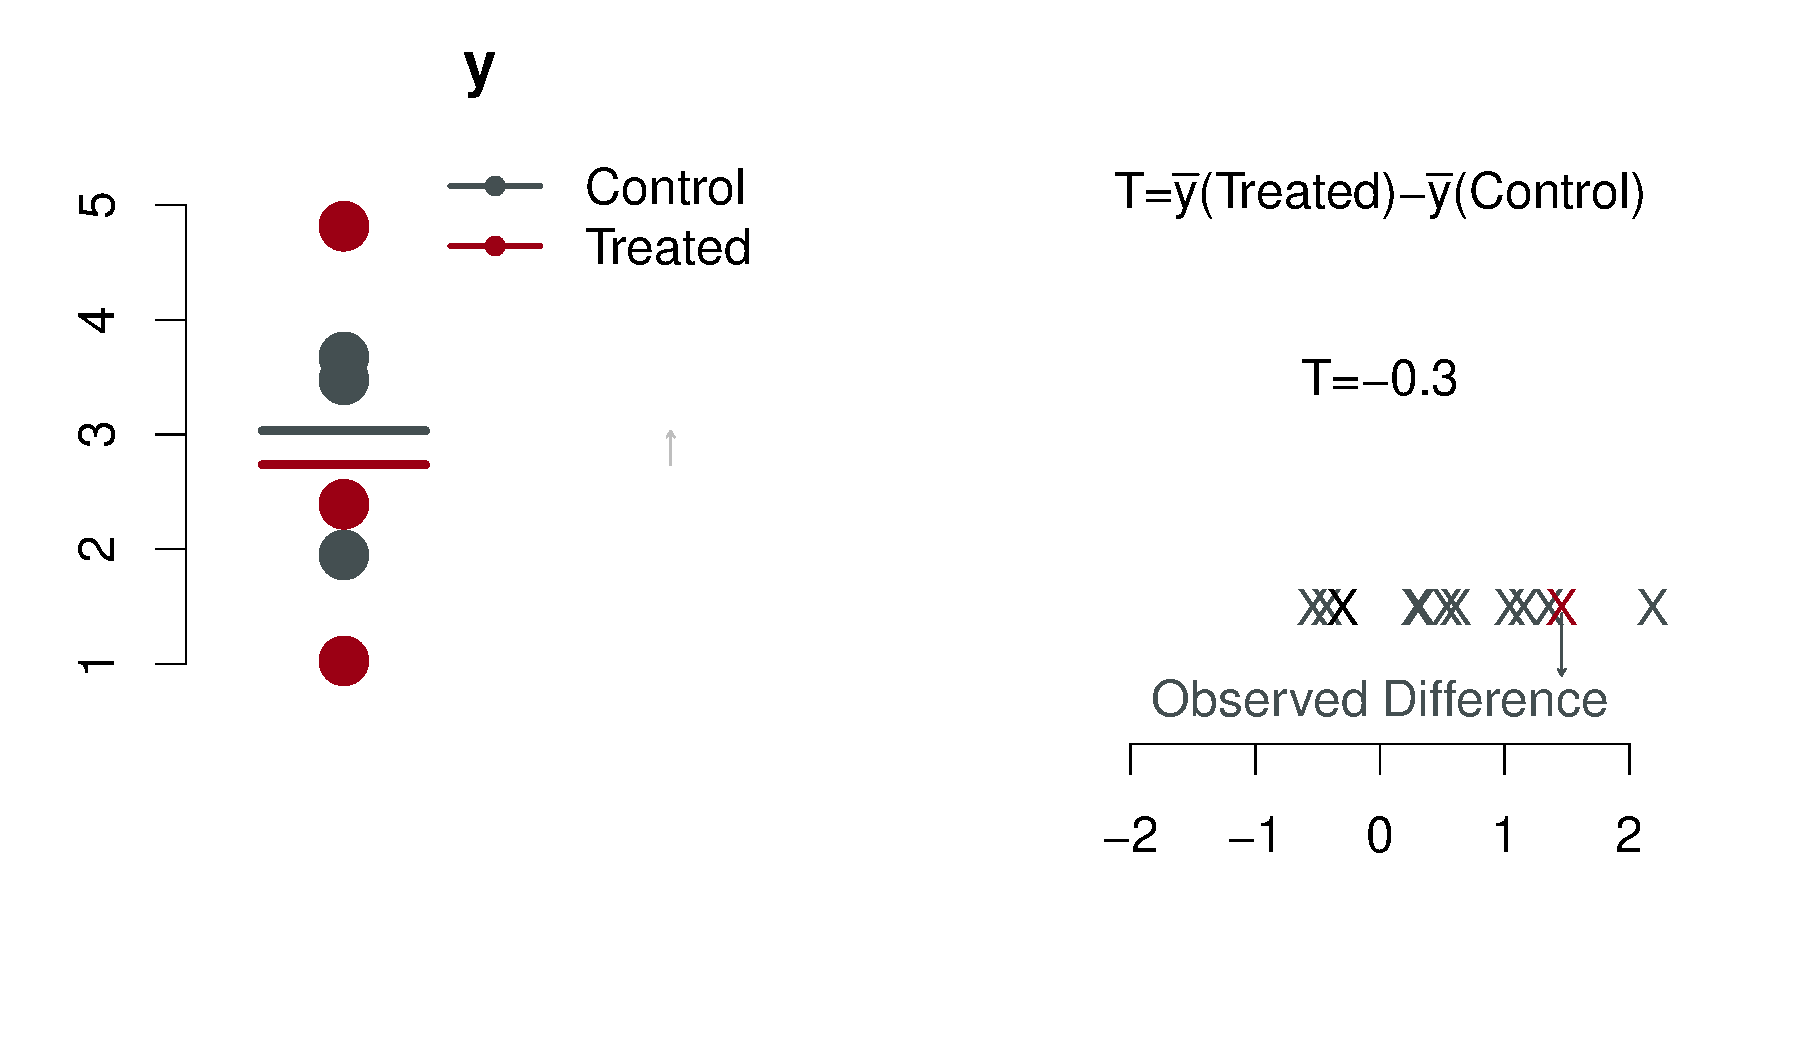
\includegraphics[width=1.1\textwidth]{figures/permsslides12} 
\end{center}
\end{frame}


\begin{frame}{A Naive approach to Permutation Testing}
 \ldots and go on with all hypothetical experiments\ldots 
\begin{center}
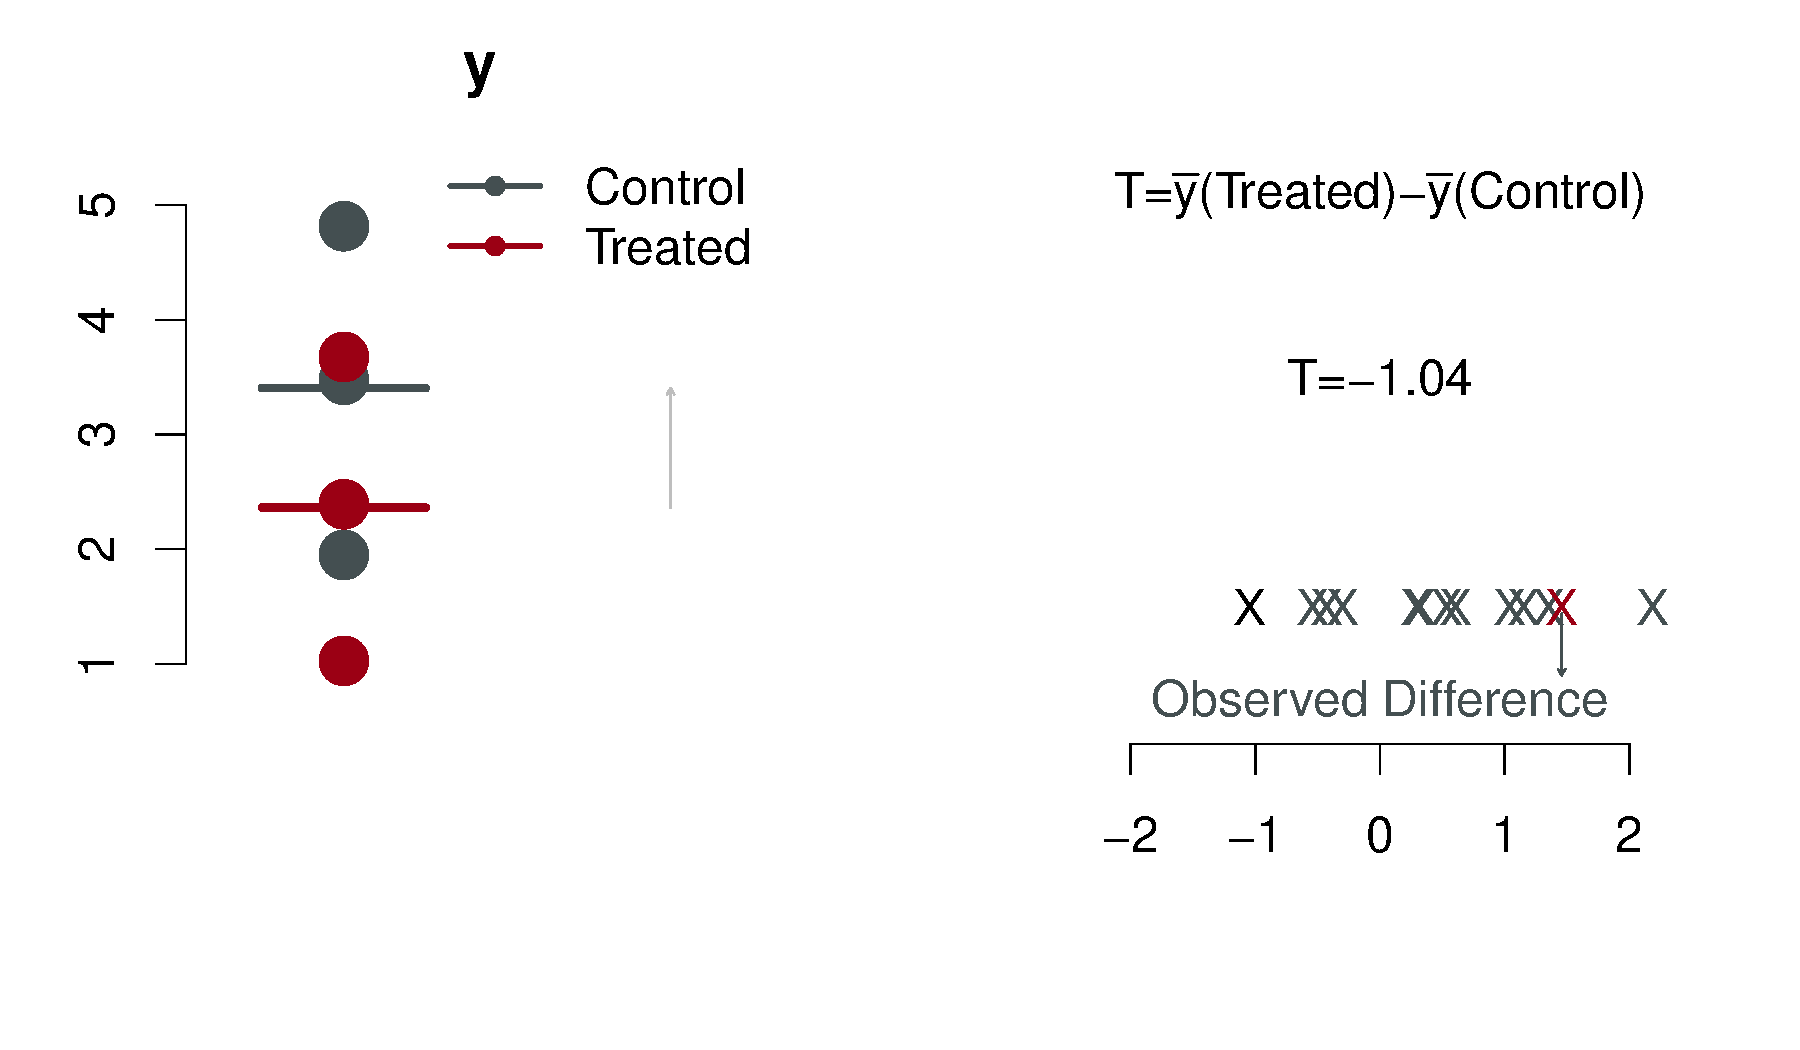
\includegraphics[width=1.1\textwidth]{figures/permsslides13} 
\end{center}
\end{frame}


\begin{frame}{A Naive approach to Permutation Testing}
 \ldots and go on with all hypothetical experiments\ldots 
\begin{center}
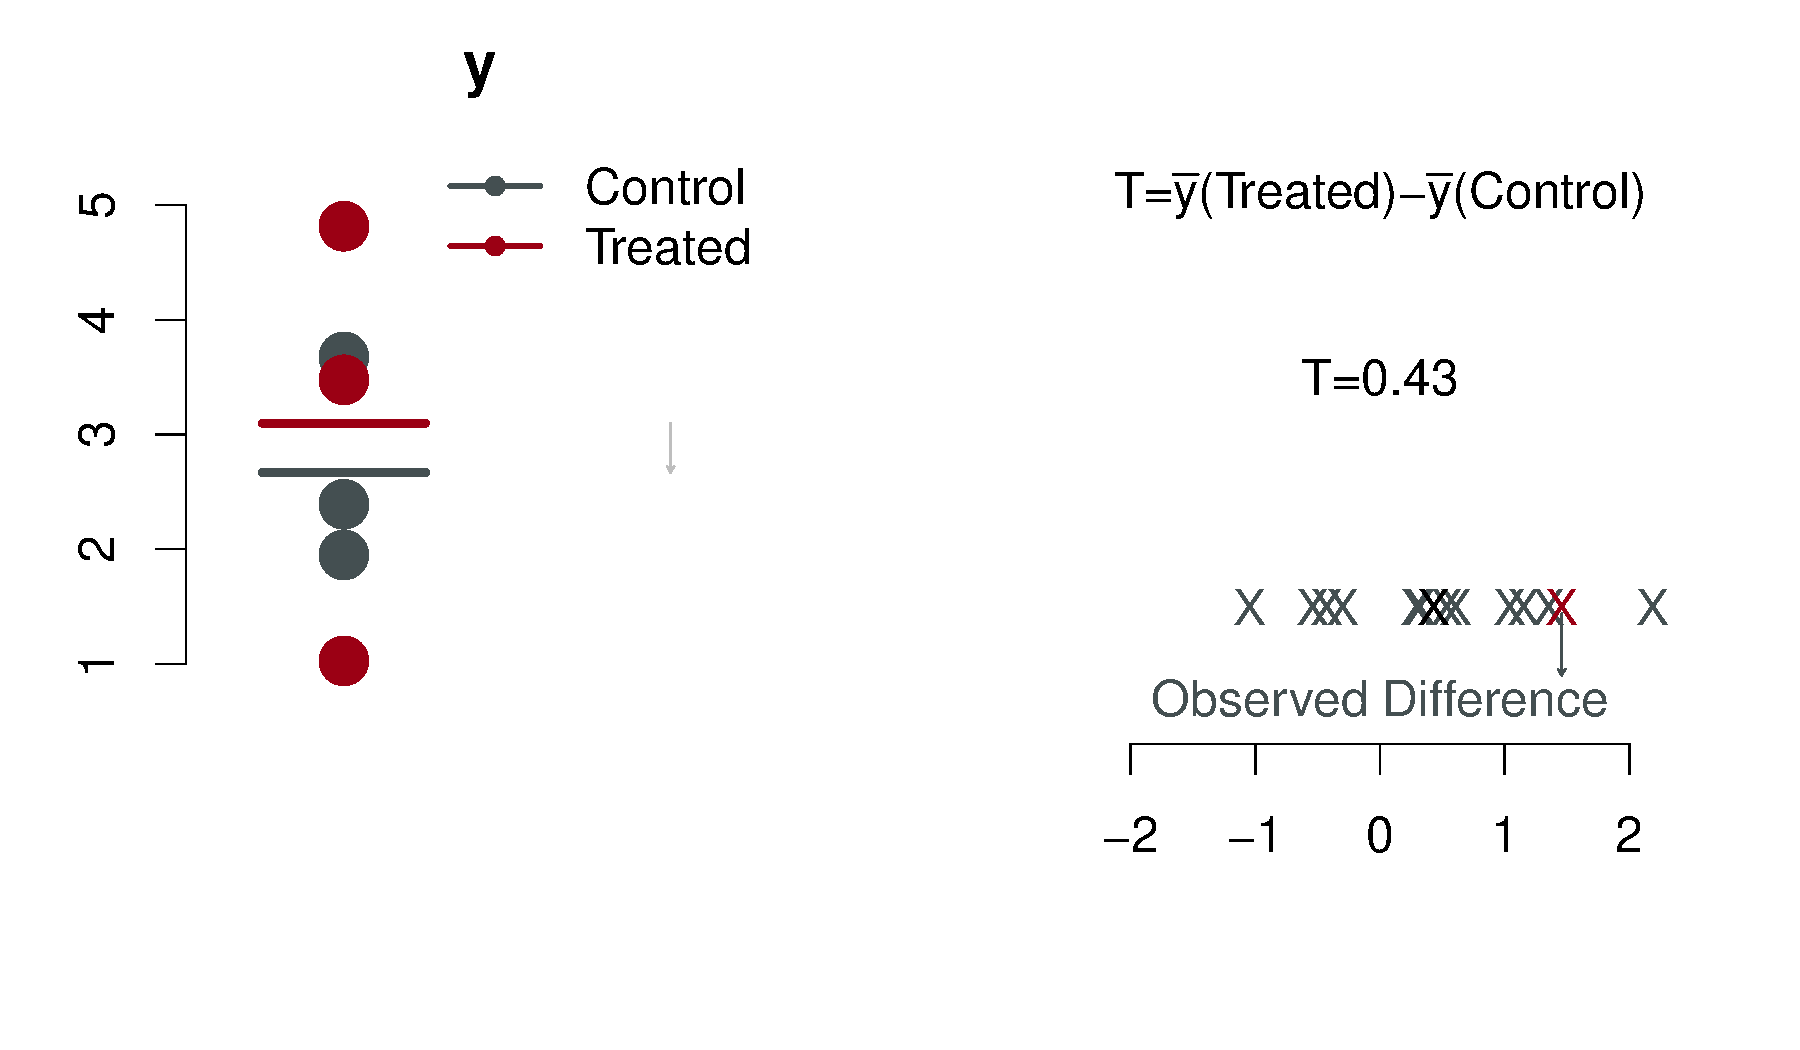
\includegraphics[width=1.1\textwidth]{figures/permsslides14} 
\end{center}
\end{frame}


\begin{frame}{A Naive approach to Permutation Testing}
 \ldots and go on with all hypothetical experiments\ldots 
\begin{center}
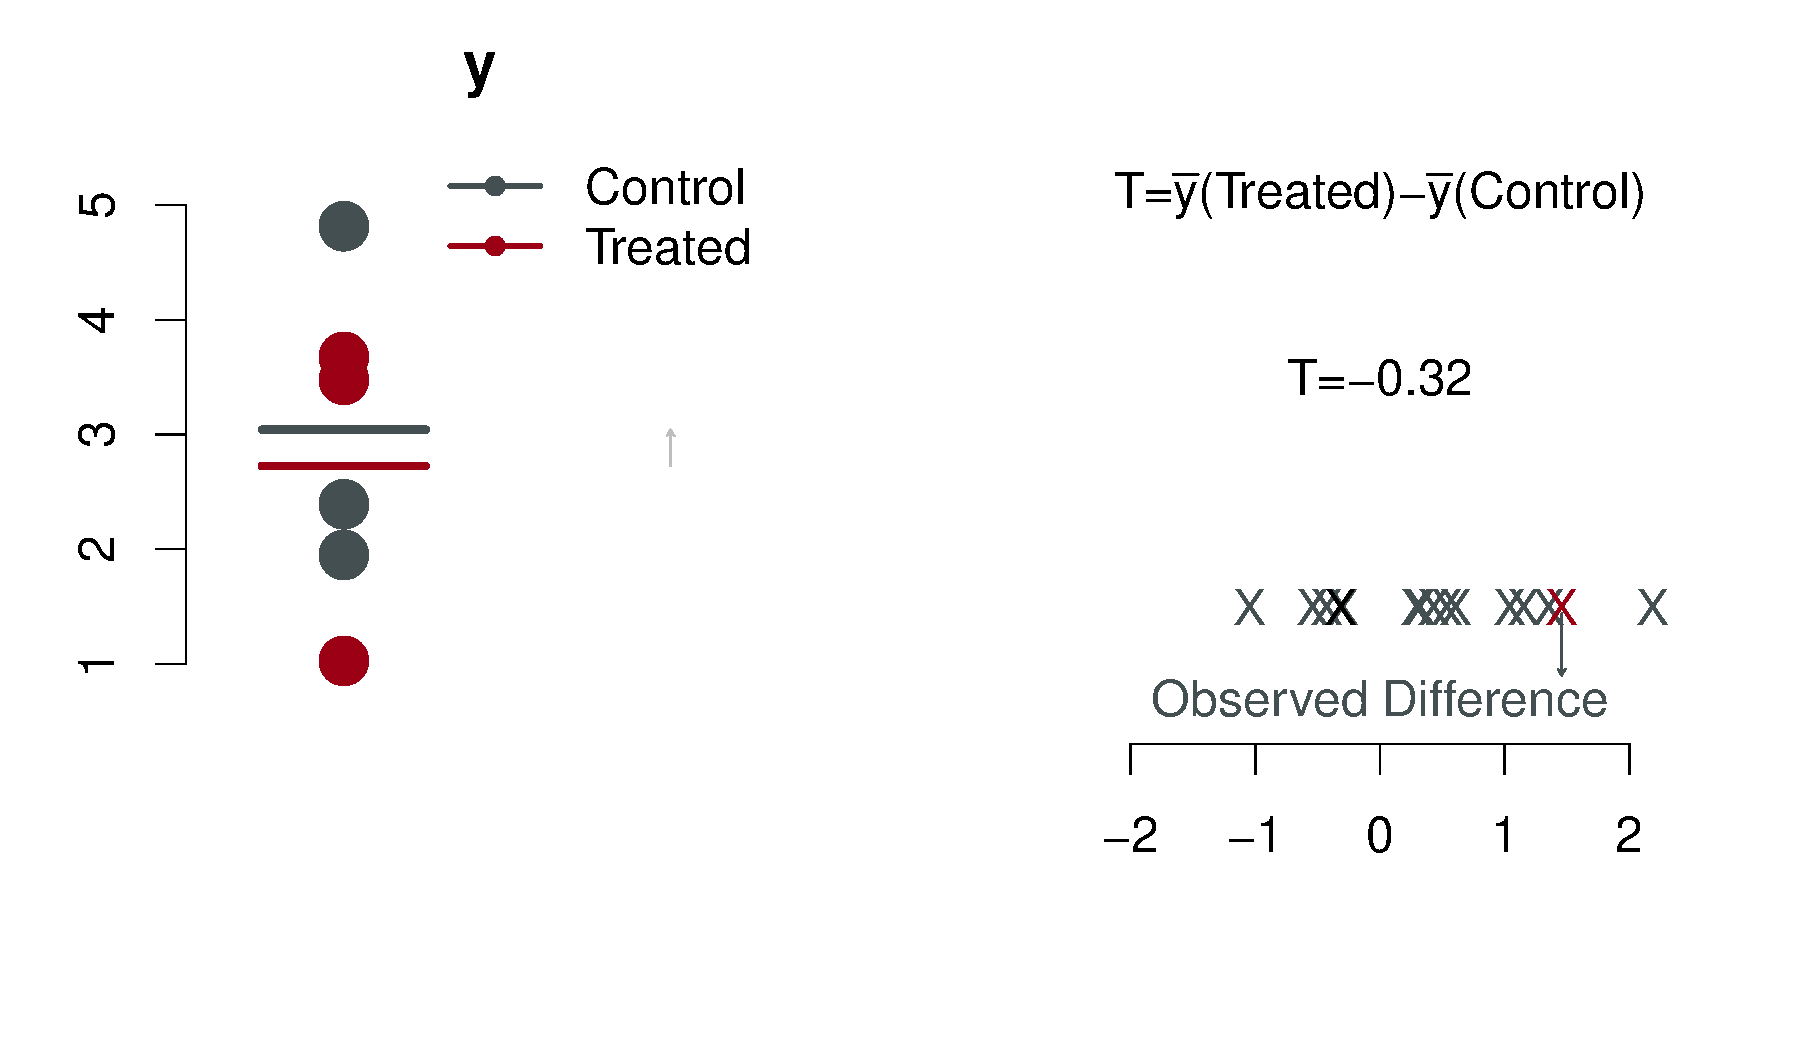
\includegraphics[width=1.1\textwidth]{figures/permsslides15} 
\end{center}
\end{frame}


\begin{frame}{A Naive approach to Permutation Testing}
 \ldots and go on with all hypothetical experiments\ldots 
\begin{center}
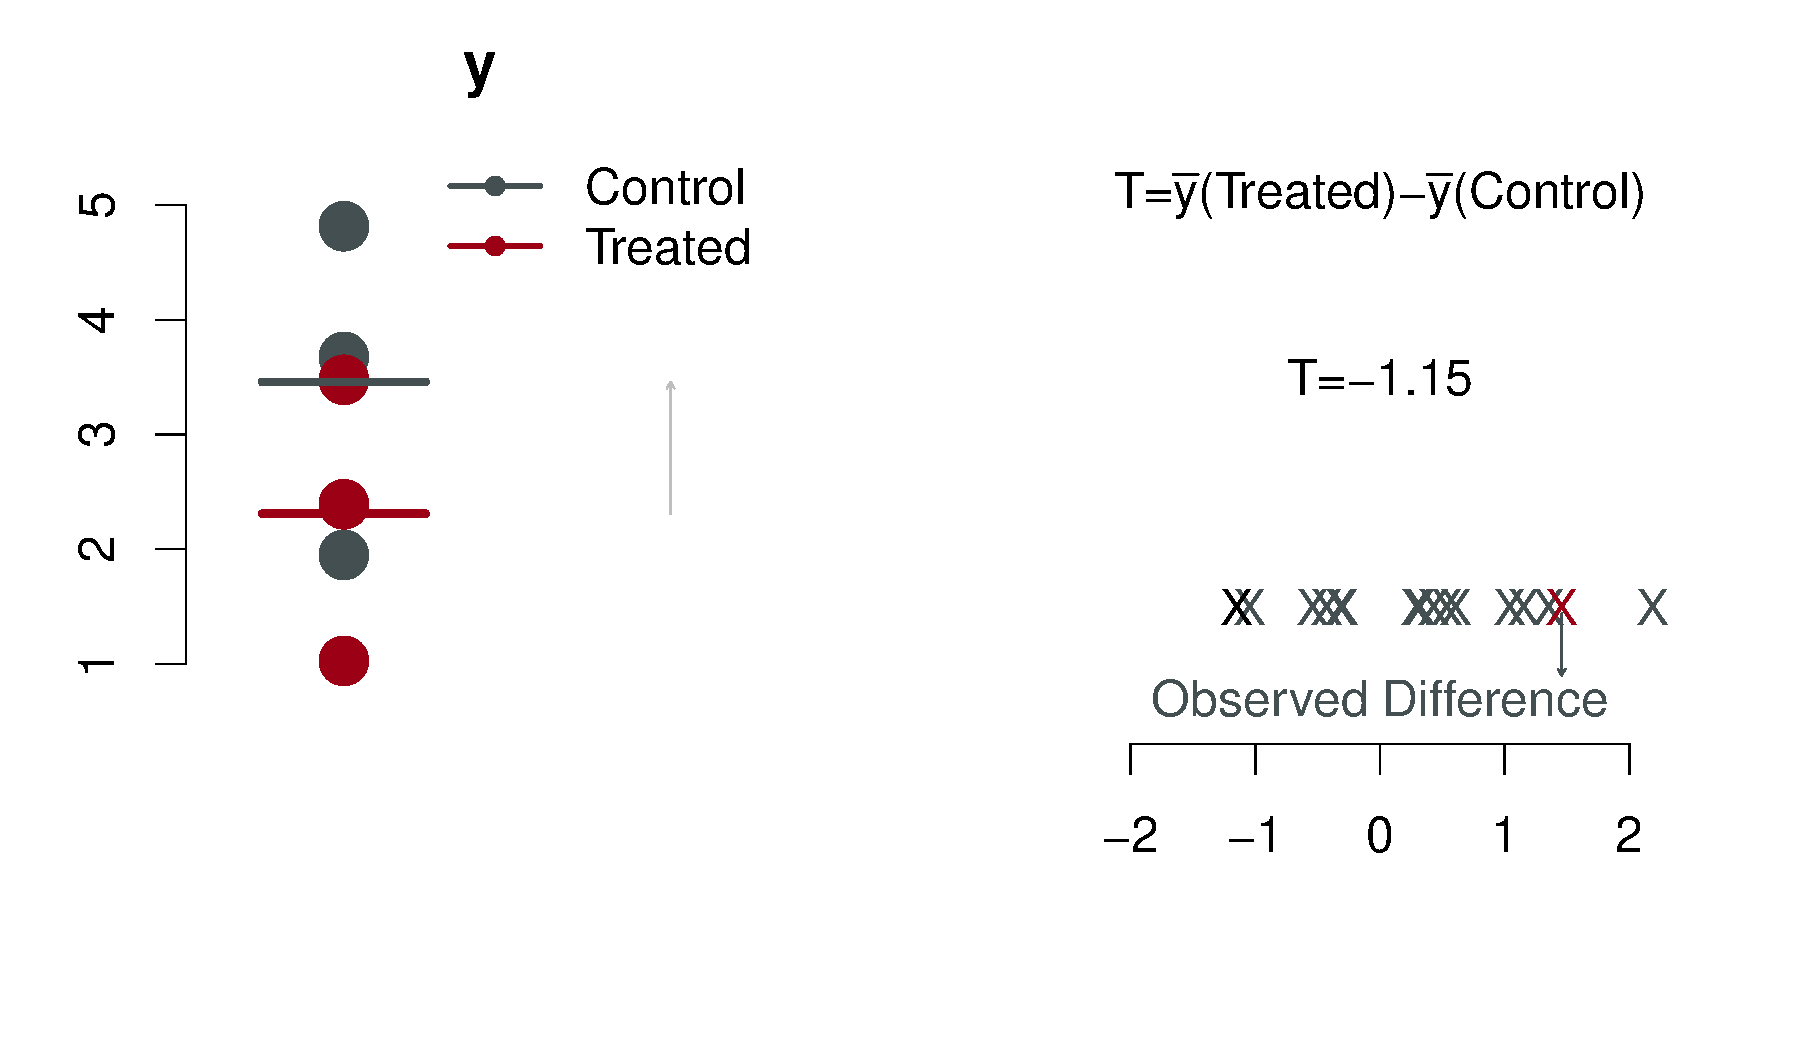
\includegraphics[width=1.1\textwidth]{figures/permsslides16} 
\end{center}
\end{frame}


\begin{frame}{A Naive approach to Permutation Testing}
 \ldots and go on with all hypothetical experiments\ldots 
\begin{center}
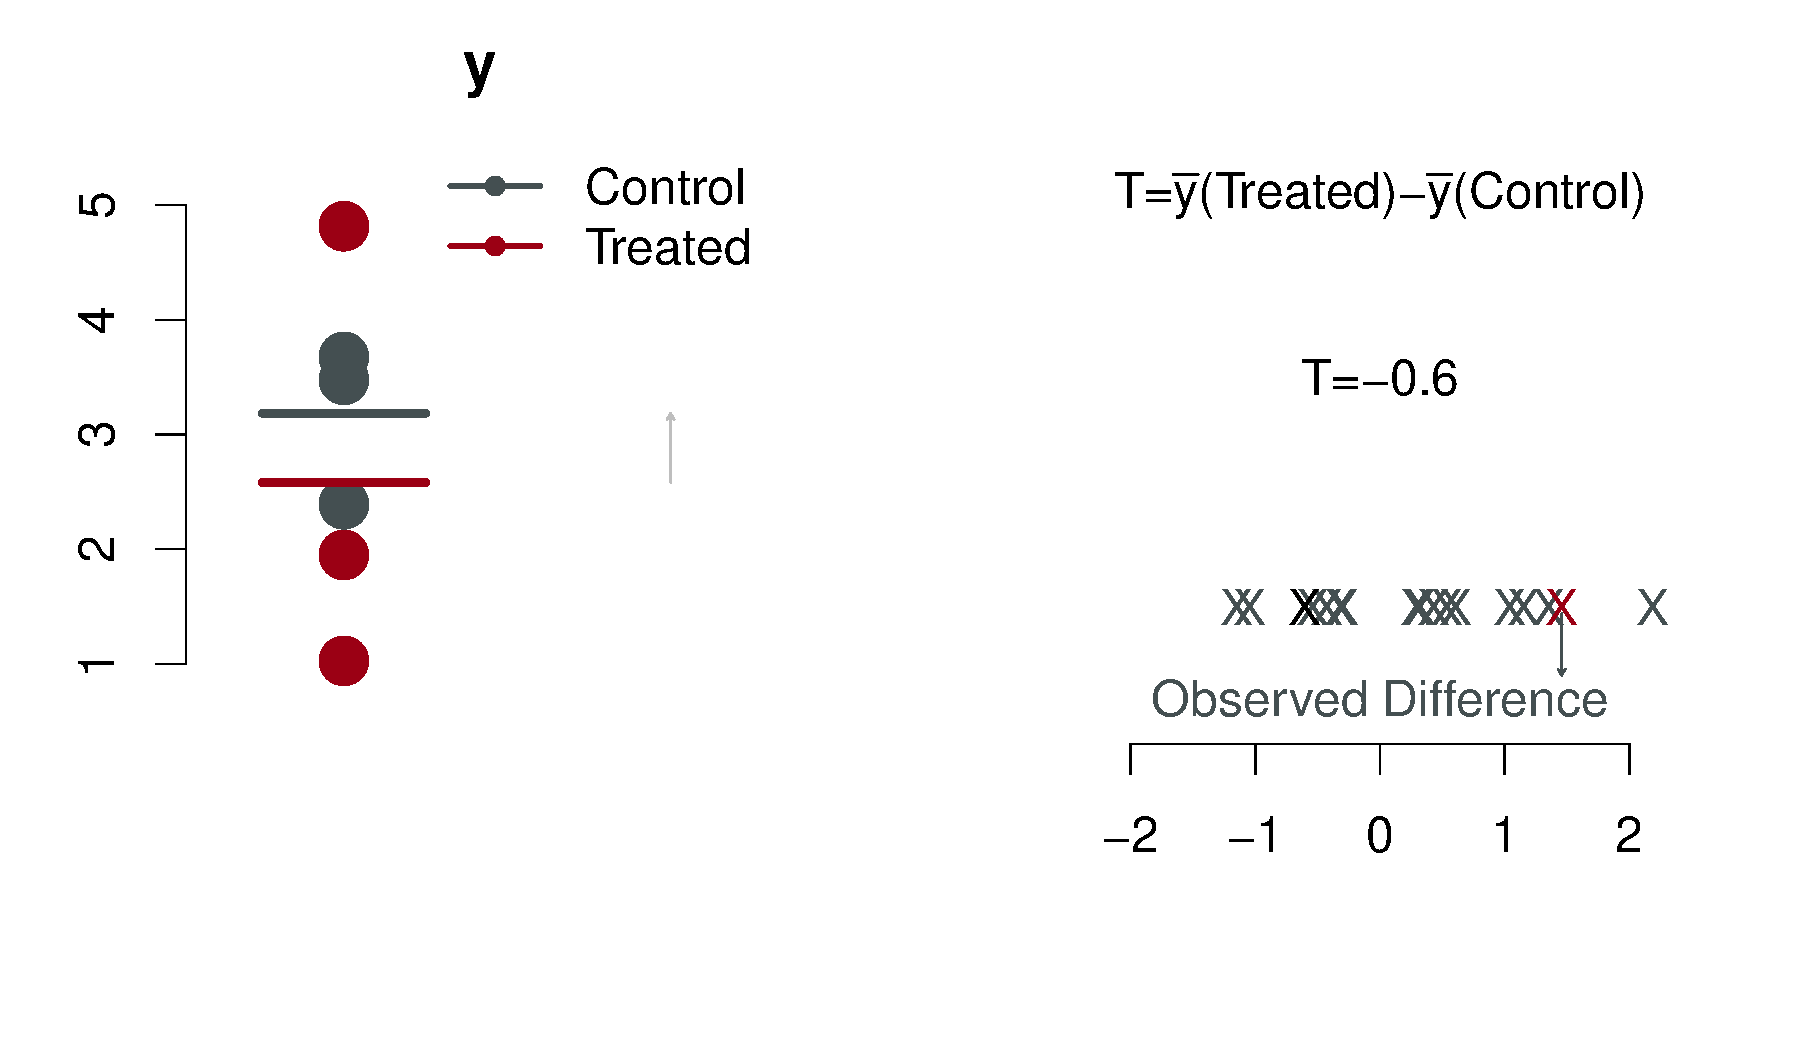
\includegraphics[width=1.1\textwidth]{figures/permsslides17} 
\end{center}
\end{frame}


\begin{frame}{A Naive approach to Permutation Testing}
 \ldots and go on with all hypothetical experiments\ldots 
\begin{center}
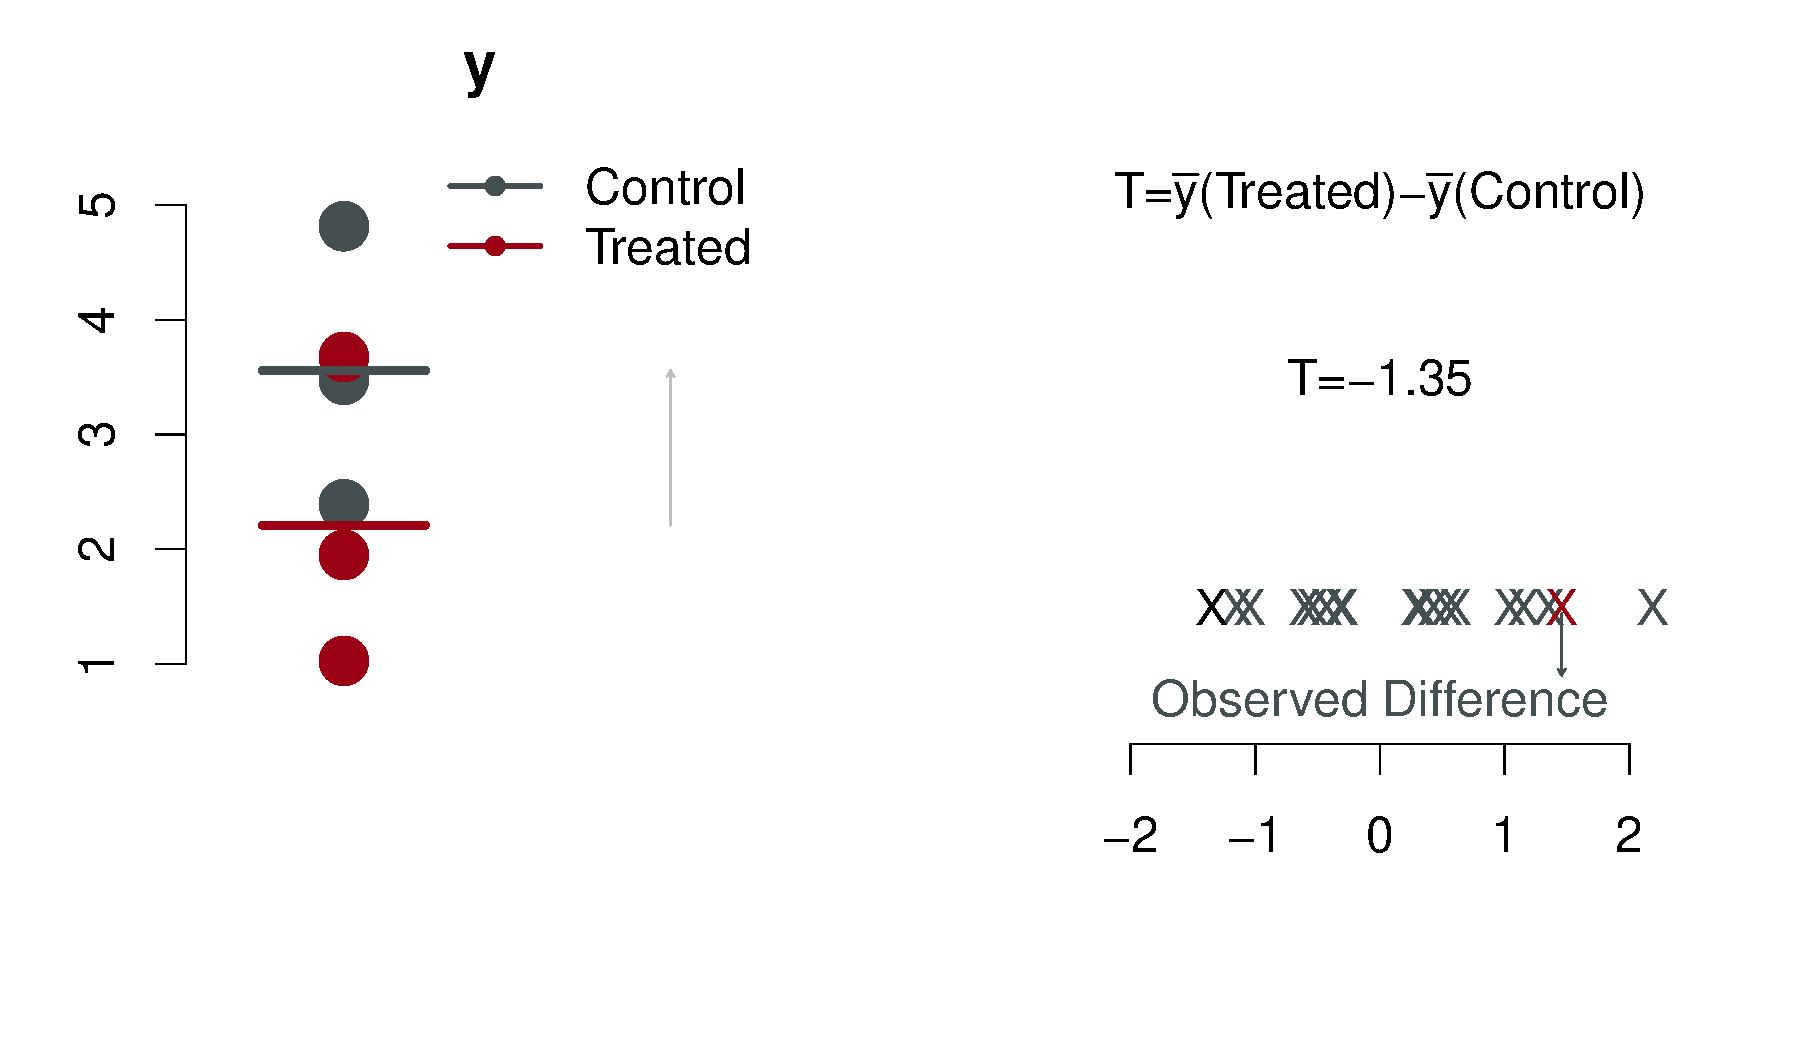
\includegraphics[width=1.1\textwidth]{figures/permsslides18} 
\end{center}
\end{frame}


\begin{frame}{A Naive approach to Permutation Testing}
 \ldots and go on with all hypothetical experiments\ldots 
\begin{center}
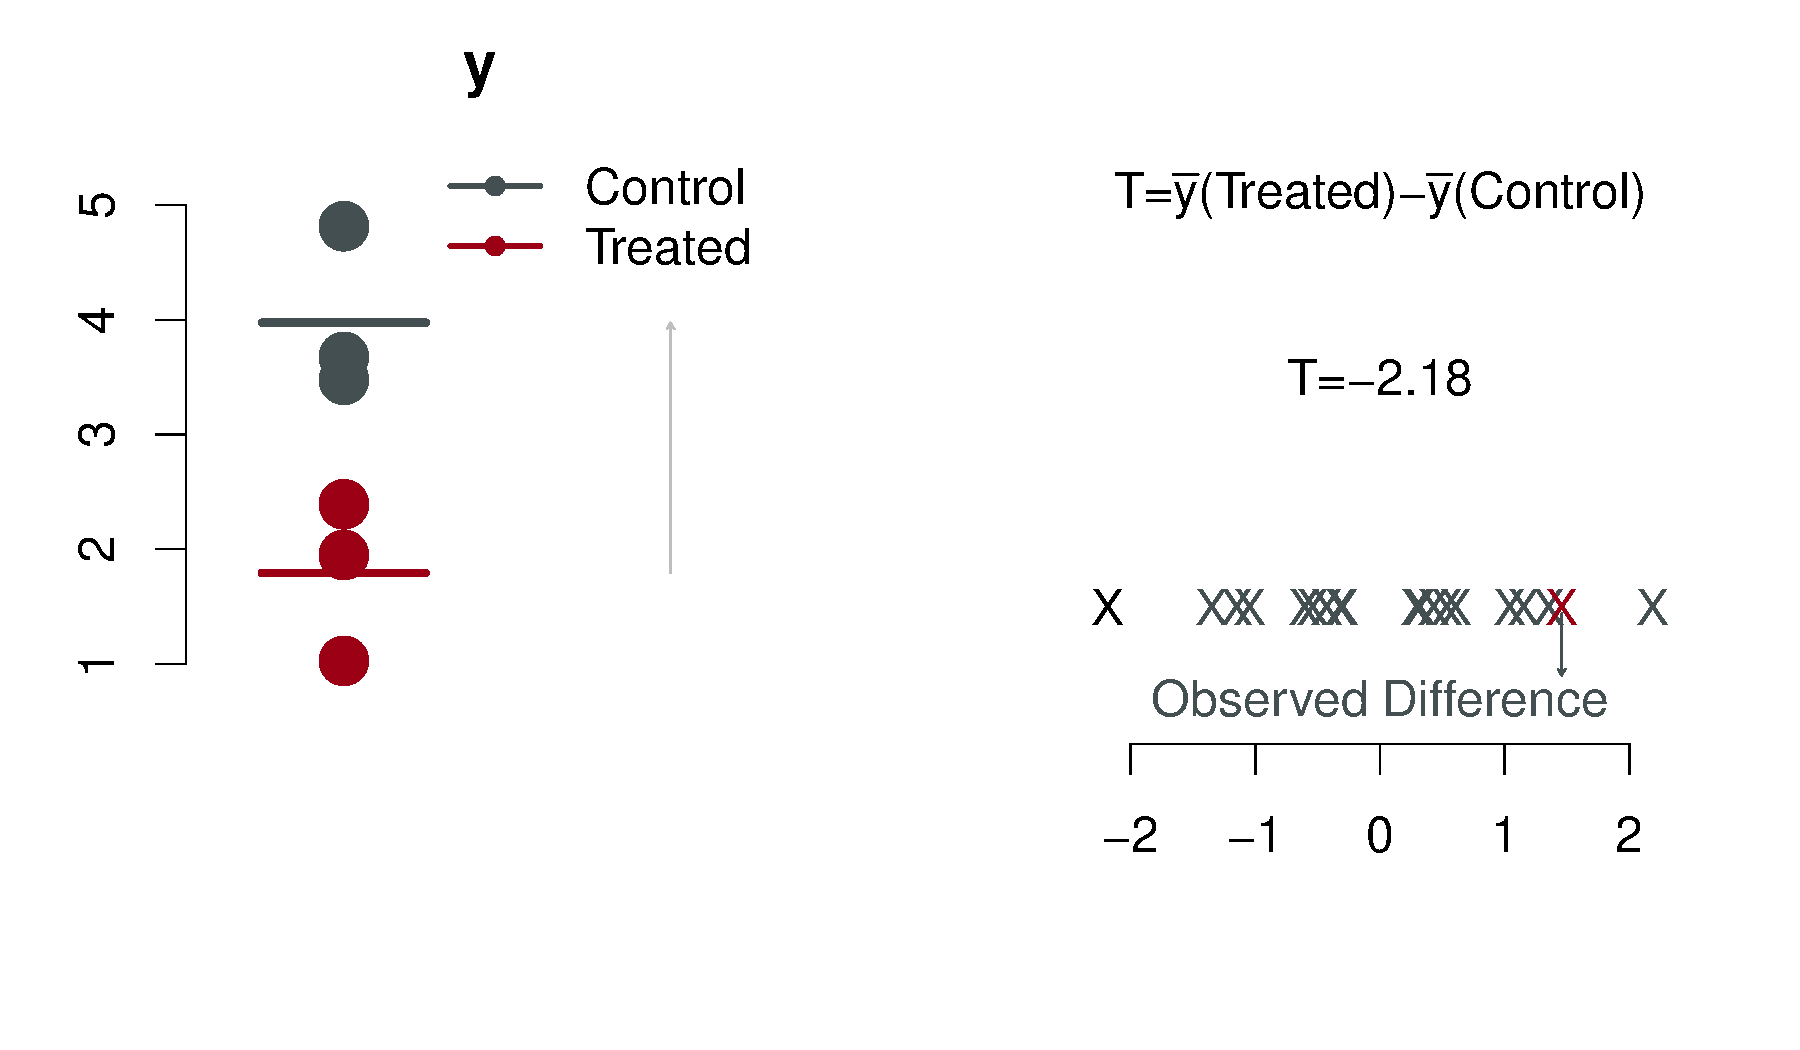
\includegraphics[width=1.1\textwidth]{figures/permsslides19} 
\end{center}
\end{frame}

\begin{frame}{A Naive approach to Permutation Testing}
 \ldots and compute the p-value!
\begin{center}
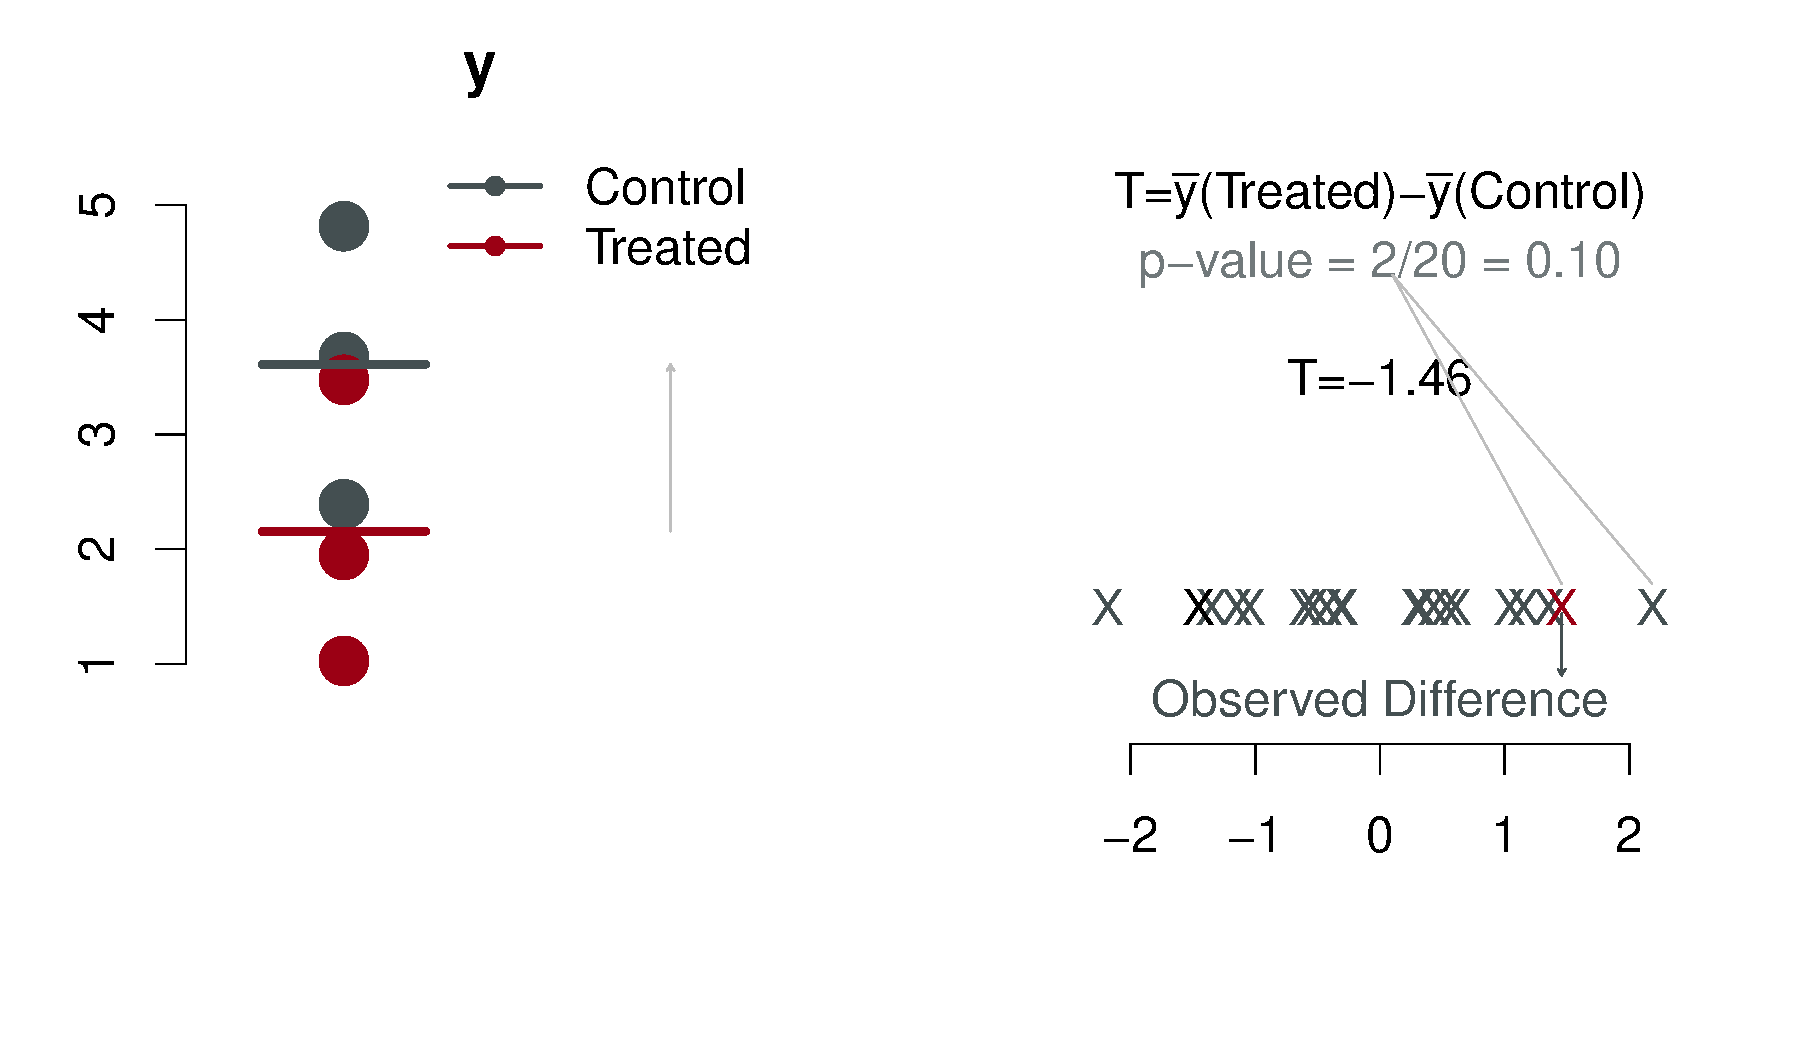
\includegraphics[width=1.1\textwidth]{figures/permsslides20} 
\end{center}
\end{frame}
%%%%%%%%%%%%%%%%%%%%%%%%%%%%%%%%
%%%%%%%%%%%%%%%%%%%%%%%%%%%%%%%%
%%%%%%%%%%%%%%%%%%%%%%%%%%%%%%%%
\begin{frame}{Summary} 
\bb{The Permutation Test:}
\begin{itemize}
\item Conditioned to observed data (i.e. the distribution of the test statistic depends on the data).
\item Under $H_0$ cases and controls have the same distribution\\(eg. they have the same  probability to get hight values),
\item explore all possible experiments that we can observe with the data (ie. exchanging cases and controls),
\item compute the p-value as the proportion of experiments providing equal or more evidence against $H_0$ with respect to observed data.

\end{itemize}
\eb
\end{frame}
%%%%%%%%%%%%%%%%%%%%%%%%%%%%%%%%
%%%%%%%%%%%%%%%%%%%%%%%%%%%%%%%%
\section{Theory (very short)}
\begin{frame}{A (slight) more formal approach}
(see also Pesarin, 2001)\\
$\yy=(y_1,y_2,\ldots,y_n)$ the vector of observed data

\medskip
\rbf{Orbit}: the set of all samples having the same likelihood under $H_0$.\\
$$\Orbit=\{\yy^*:\ f(\yy^*)=f(\yy) \}$$
(and $|\Orbit|$ number of elements of $\Orbit$)

\medskip

If we assume exchangeability of observations, then:
$$\Orbit=\{\textrm{all permutations of the observed data }\yy\} = \{\yy^*:\pi^*\circ\yy\}$$
($\pi^*\in \Pi,\ \Pi$ set of all possible permutations)

\end{frame}
%%%%%%%%%%%%%%
\begin{frame}{A (slight) more formal approach}

{\bf Remark}: exchangeable observations: $f(y_1,y_2)=f(y_2,y_1)$. \\ It implies observations:
\bi
\item are {\bf identically distributed}\\ t-test and linear models assume normality, only asymptotic control of the tye I error
\item have the {\bf same dependence}\\ 
t-test and linear models assume independence, which is just a special case, i.e. more stringend assumptions 
\ei

\end{frame}
%%%%%%%%%%%%%%
\begin{frame}{A (slight) more formal approach}

\rbf{p-value}: proportion of experiments providing equal or more evidence against $H_0$ with respect to observed data.

\medskip
To compute it, we need the \rbf{Orbit $\Orbit$} and a \pause \\
\rbf{Test statistic} (\rbf{$T$}:  $\mathbb{R}^n\to\mathbb{R}$) quantifies the evidence against $H_0$
\bi
\item higher values provide more evidence against $H_0$
\item compute a test statistic for each element of the Orbit $\Orbit$, \\ this induces an ordering on $\Orbit$.
\ei
In our example: $T=\bar{y}(Treated)-\bar{y}(Control)$ is the difference in mean, higher the difference, higher the evidence for $H_1$. 
\end{frame}
%%%%%%%%%%%%%%
\begin{frame}{A (slight) more formal approach}

$$f(\yy^*|\Orbit)=\frac{f(\yy^*\cap\Orbit)}{f(\Orbit)}=
\frac{f(\yy^*)}{f(\Orbit)}=
\frac{f(\yy^*)}{f(\cup_{y\in\Orbit}y)}=\frac{1}{|\Orbit|}\ \forall\ \yy^*\in \Orbit$$
i.e. each permutation is equally likely in the Orbit $\Orbit$.

\medskip
The \rbf{p-value}:
\begin{eqnarray*}
&&P(T(\yy^*)\geq T(\yy) | \yy^*\in\Orbit, H_0)=\\
&=&\int_{T(\yy)}^{+\infty} f(T(\yy^*))dT(\yy^*)=\\
&=&\sum_{\yy^*\in\Orbit} I(T(\yy^*)\geq T(\yy))/|\Orbit|\ \ \ \ \forall\Orbit
\end{eqnarray*}

%  For this reason, permutation tests are conditional procedures.
\end{frame}
%%%%%%%%%%%%%%%%%%%%%%%%%%%%%%%%
%%%%%%%%%%%%%%%%%%%%%%%%%%%%%%%%
\bfr{The package flip}
It is on CRAN and on github (https://github.com/livioivil/flip)

To install the github version type (in R):\\
{\tt 
library(devtools)\\
install\_github('livioivil/flip')}

\end{frame}
%%%%%%%%%%%%%%%%%%
\bfr{Seeds data (Pesarin, 2001)}
Standard fertilizer ($grp=0$) vs New fertilizer ($grp=1$)

Total weight of the plant and average leaves length is recorded.
\begin{center}
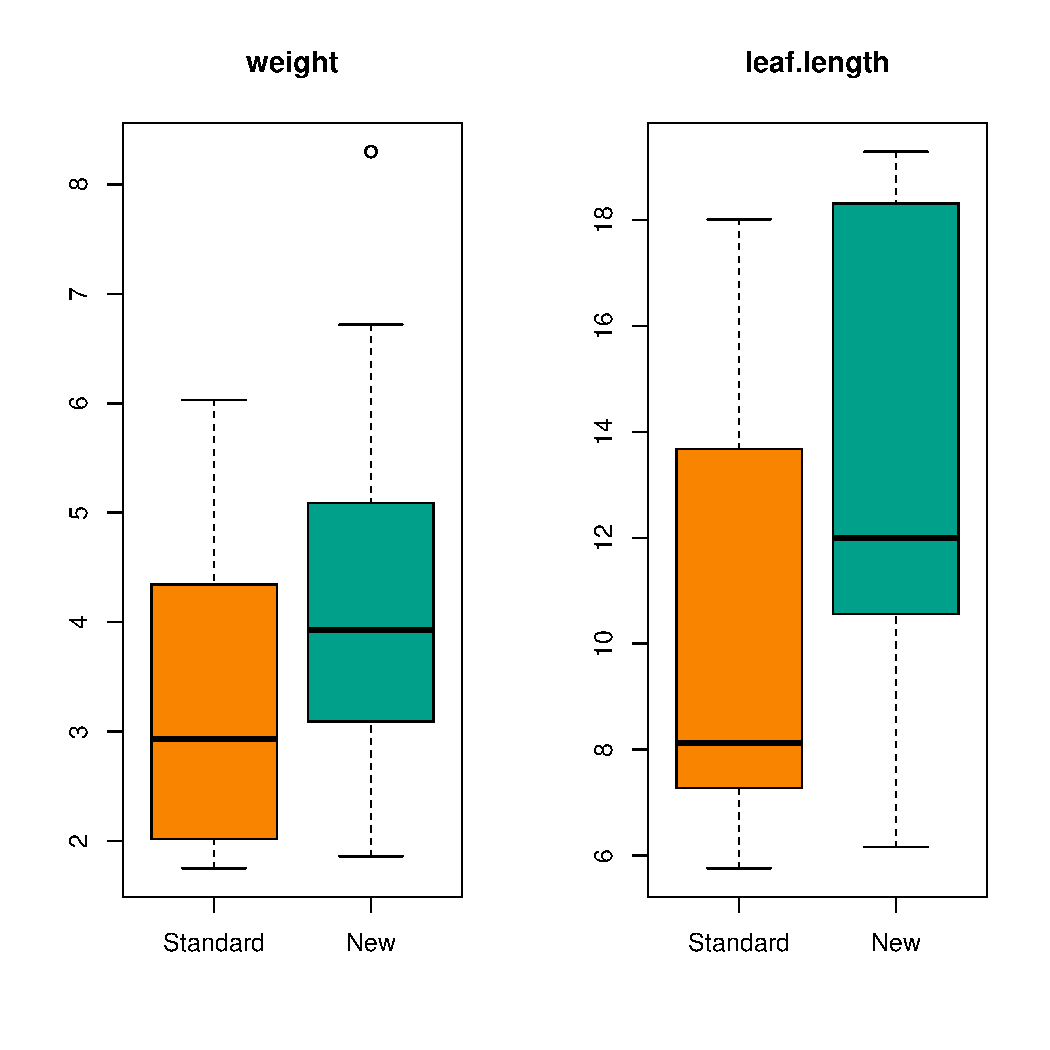
\includegraphics{figures/boxplots}
\end{center}
\end{frame}
%%%%%%%%%%%%%%%%%%
\bfr{Hypothesis testing}
About weight:
\bi
\item $H_0(weight): F(weight|grp=0)=F(weight|grp=1)$
\item[] vs
\item $H_1(weight): F(weight|grp=0)> F(weight|grp=1)$
\ei
\bigskip
And about leaf length:
\bi
\item $H_0(leaf.len): F(leaf.len|grp=0)=F(leaf.len|grp=1)$
\item[] vs
\item $H_1(leaf.len): F(leaf.len|grp=0)> F(leaf.len|grp=1)$
\ei
\end{frame}
\bfr{Hypothesis testing}

{\tt res=flip(.$\sim$ grp, data=seeds, tail=1)}
% latex table generated in R 3.2.0 by xtable 1.7-4 package
% Mon Nov 30 13:14:19 2015
\begin{table}[ht]
\centering
\begin{tabular}{rlrlr}
  \hline
 & Test & Stat & tail & p-value \\ 
  \hline
weight & t & 1.320 & $>$ & 0.098 \\ 
  leaf.length & t & 2.061 & $>$ & 0.030 \\ 
   \hline
\end{tabular}
\end{table}
  
together with some visualization
{\tt hist(res)}
\begin{center}
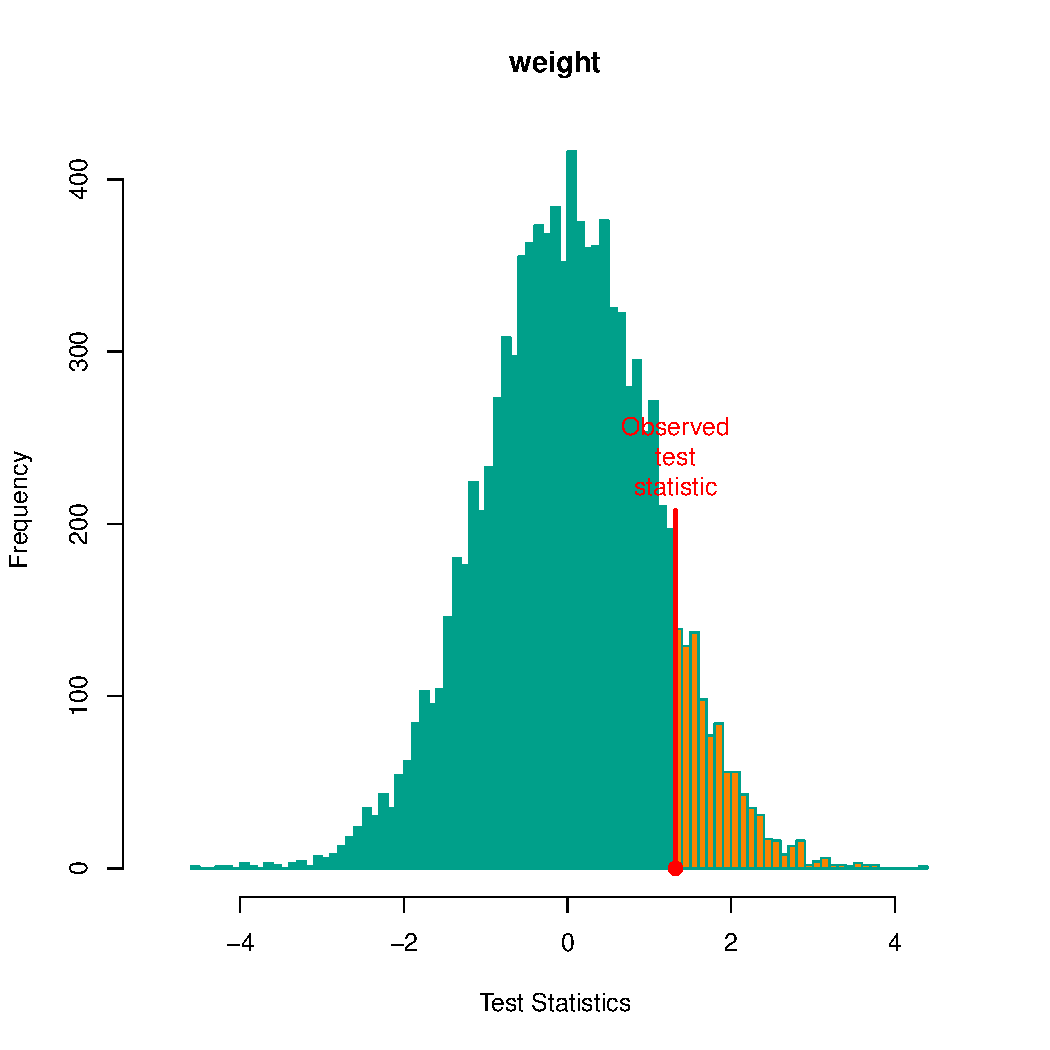
\includegraphics[width=6cm]{figures/hist1}
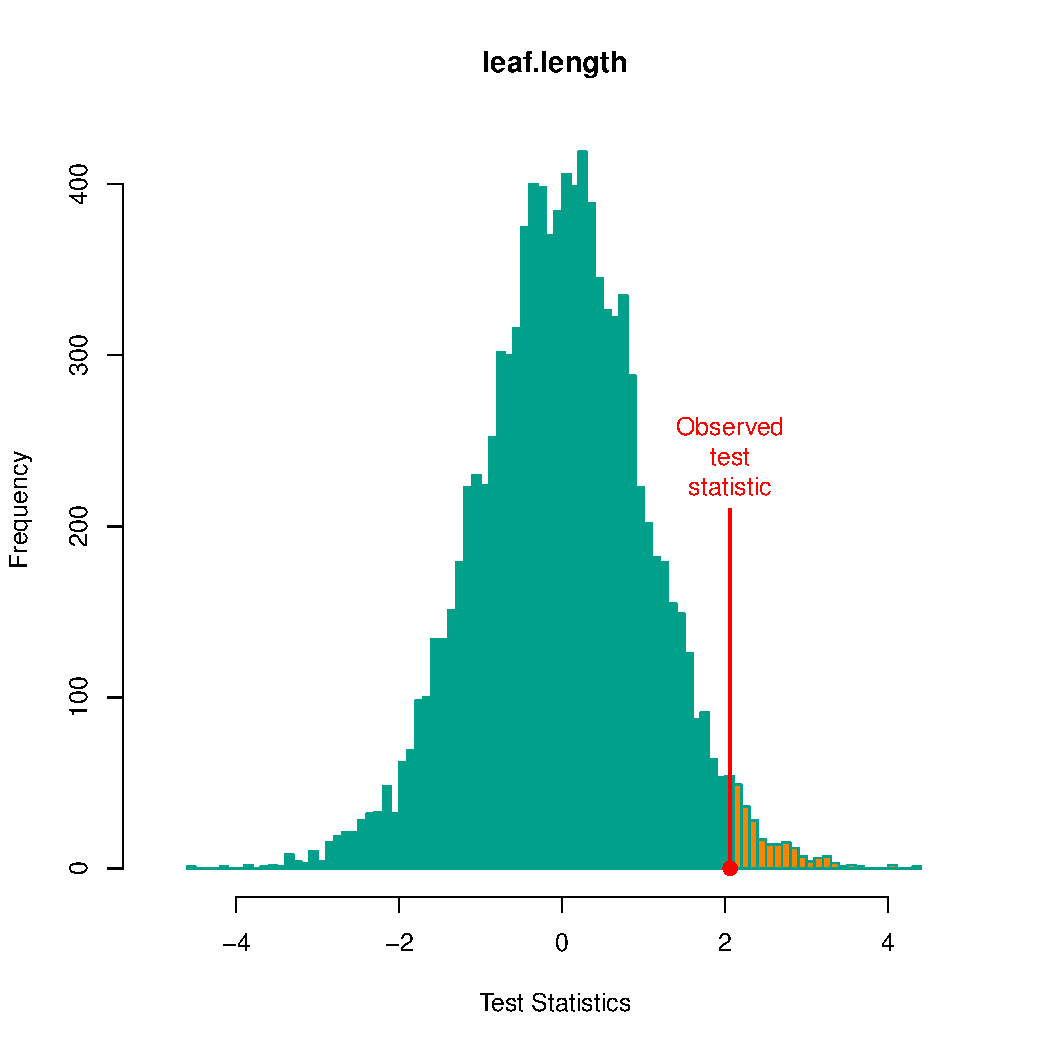
\includegraphics[width=6cm]{figures/hist2}
\end{center}
\end{frame}

%%%%%%%%%%%%%%%%%%%%%%%%%%%%%%%%
%%%%%%%%%%%%%%%%%%
\bfr{Two-tailed tests}
About weight:
\bi
\item $H_0(weight): F(weight|grp=0)=F(weight|grp=1)$
\item[] vs
\item $H_1(weight): F(weight|grp=0)\rbf{\neq} F(weight|grp=1)$
\ei
\bigskip
And about leaf length:
\bi
\item $H_0(leaf.len): F(leaf.len|grp=0)=F(leaf.len|grp=1)$
\item[] vs
\item $H_1(leaf.len): F(leaf.len|grp=0)\rbf{\neq} F(leaf.len|grp=1)$
\ei
\end{frame}
\bfr{Two-tailed tests}

{\tt res=flip(.$\sim$ grp, data=seeds, tail=0)}
% latex table generated in R 3.2.0 by xtable 1.7-4 package
% Mon Nov 30 13:14:19 2015
\begin{table}[ht]
\centering
\begin{tabular}{rlrlr}
  \hline
 & Test & Stat & tail & p-value \\ 
  \hline
weight & t & 1.320 & $><$ & 0.202 \\ 
  leaf.length & t & 2.061 & $><$ & 0.049 \\ 
   \hline
\end{tabular}
\end{table}
  
Also very negative values provide evidence against $H_0$
\begin{center}
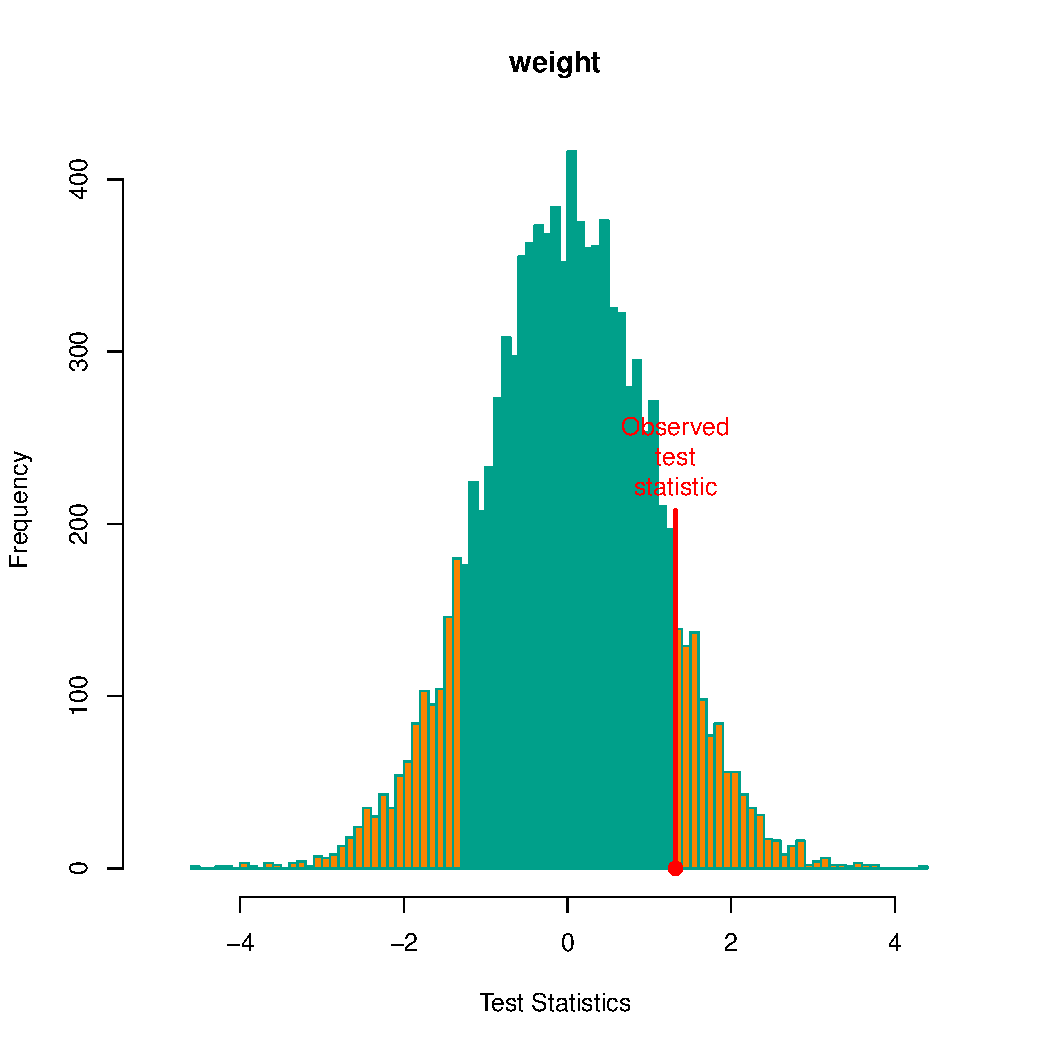
\includegraphics[width=6cm]{figures/hist3}
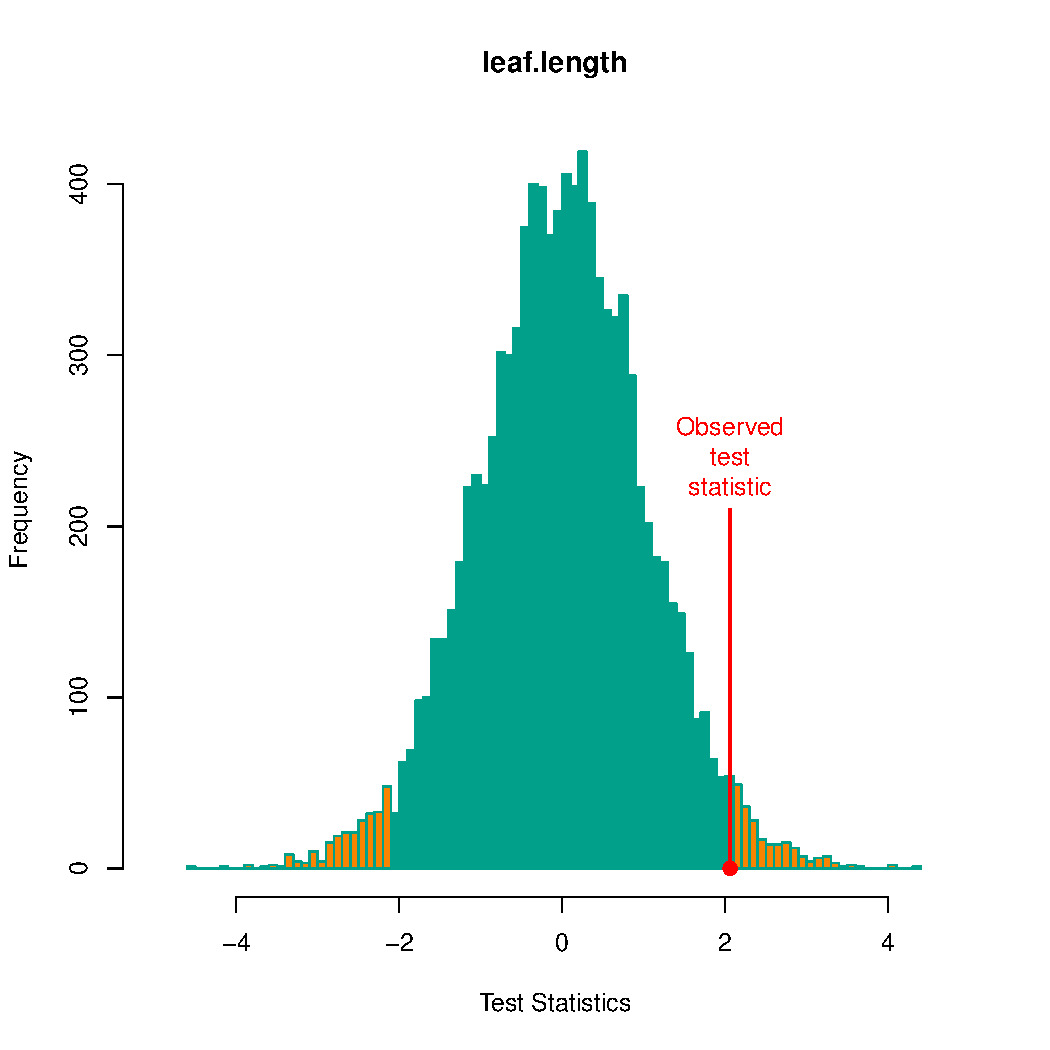
\includegraphics[width=6cm]{figures/hist4}
\end{center}
\end{frame}

%%%%%%%%%%%%%%%%%%%%%%%%%%%%%%%%
\begin{frame}{Properties} 
\bi
\item Exact control of the Type I Error:
$P(p\leq\alpha|H_0)<\alpha\ \forall\ \textrm{(attainable)} \alpha$
\item Consistency: $P(p\leq\alpha|H_1)\to 1$ when $n\to\infty$
\item Converges to parametric counterpart (i.e. asymptotic optimality if the parametric test is optimal)
\ei
\bb{Remark}
The number of possible permutations (size of the Orbit $|\Orbit|$) is often huge, we can not compute the test statistic for all elements.\\
Common use to sample from the Orbit (i.e. randomly permute the labels $B$ times).\\
The properties remain the same.
\eb
\end{frame}
%%%%%%%%%%%%%%%%%%%%%%%%%%%%%%%%
%%%%%%%%%%%%%%%%%%%%%%%%%%%%%%%%
\bfr{Simulation: normal distribution}
\bi
\item Comparison of Two groups (labels A, B) of size 5 
\item $y_i\sim N(0,1)$
  \item[] 
\bi
\item $H_0:f(y|grp=A)=f(y|grp=B)$
  \item $H_0:f(y|grp=A)\neq f(y|grp=B)$\\ 
(i.e. two-sided alternatives)
\ei
\item 10000 replications
\item 1000 random permutations for each test
\ei
\end{frame}
%%%%%%%%%%%%%%%%%
\bfr{Simulation: $H_0$}
\begin{center}
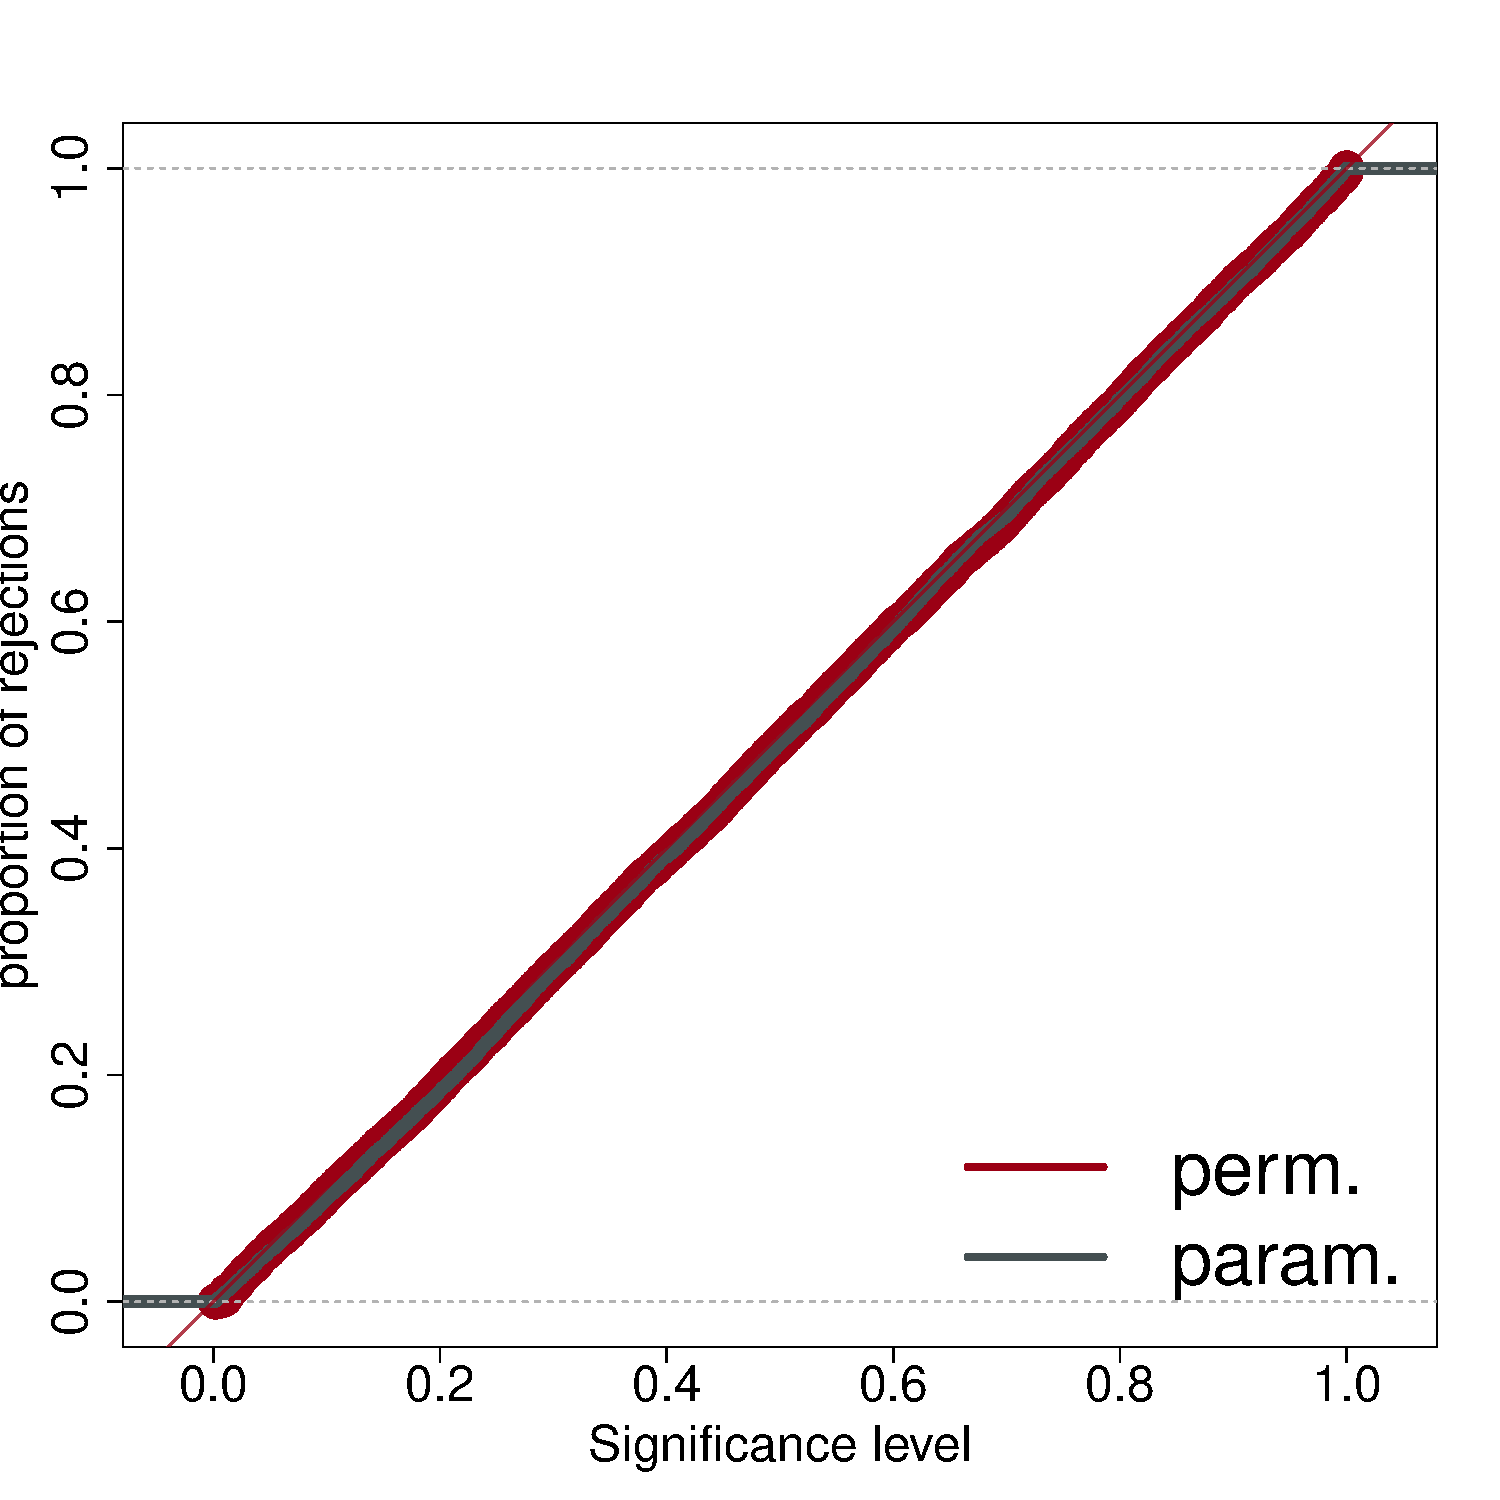
\includegraphics[width=0.55\textwidth]{figures/sim0} 
\end{center}

\begin{table}[ht]
\centering
\begin{tabular}{rrrrrr}
\hline
Empirical Type I error & $\leq$0.01 & $\leq$0.05 & $\leq$0.1 & $\leq$0.5 & $\leq$0.75 \\ 
\hline
Permutation & 0.00 & 0.05 & 0.09 & 0.49 & 0.74 \\ 
Paramatric t.test & 0.01 & 0.04 & 0.09 & 0.49 & 0.75 \\ 
\hline
\end{tabular}
\end{table}
\end{frame}
%%%%%%%%%%%%%%%%%%%%%%%%%%%%%%%%
  \bfr{Simulation: $H_1$}
now $(y|grp=A)\sim N(0,1)$, $(y|grp=B)\sim N(2,1)$
  \begin{center}
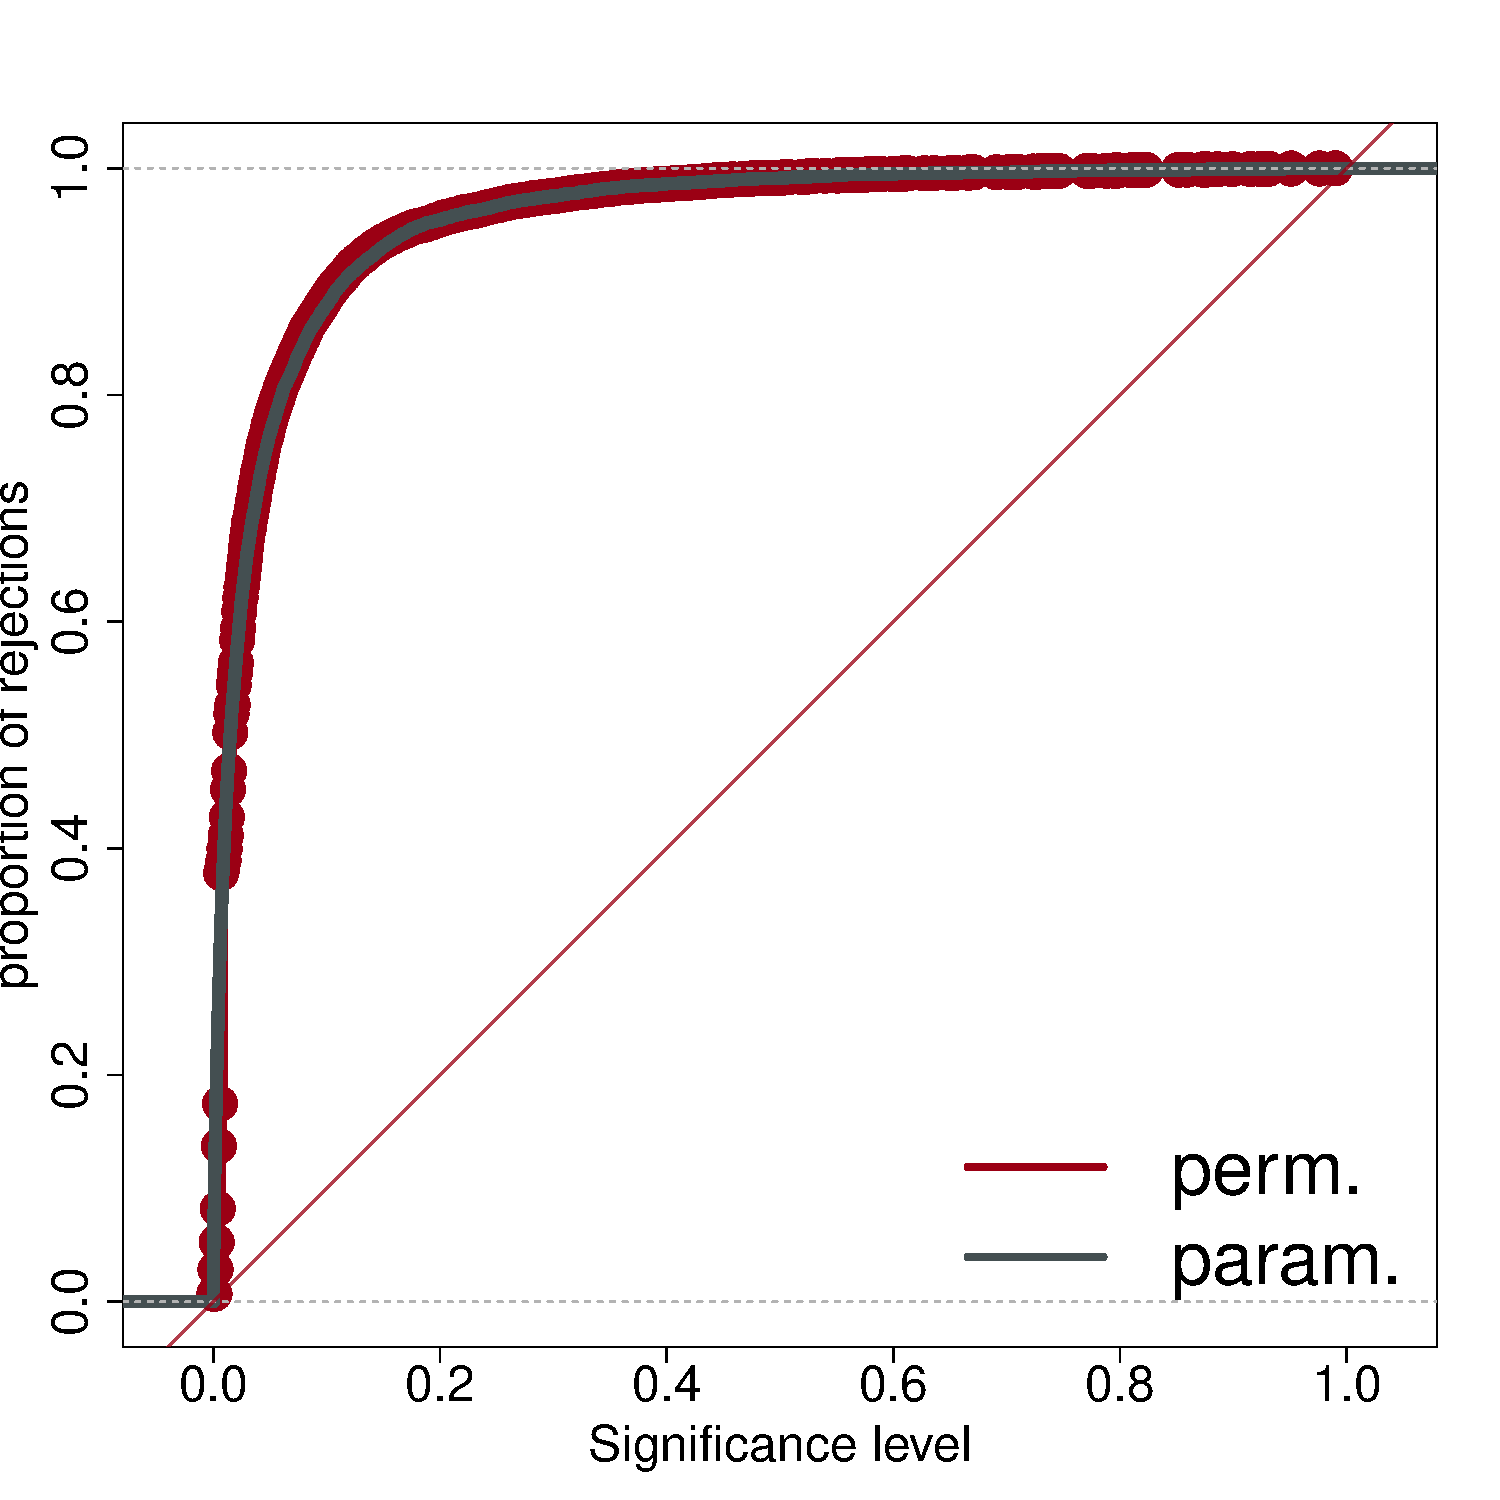
\includegraphics[width=0.55\textwidth]{figures/sim1} 
\end{center}

\begin{table}[ht]
\centering
\begin{tabular}{rrrrrr}
\hline
Empirical Power & $\leq$0.01 & $\leq$0.05 & $\leq$0.1 & $\leq$0.5 & $\leq$0.75 \\ 
\hline
Permutation       & 0.40 & 0.78 & 0.89 & 0.99 & 1.00 \\ 
Paramatric t.test & 0.41 & 0.77 & 0.88 & 0.99 & 1.00 \\
\hline
\end{tabular}
\end{table}
\end{frame}
%%%%%%%%%%%%%%%%%%%%%%%%%%%%%%%%
  %%%%%%%%%%%%%%%%%%%%%%%%%%%%%%%%%
\bfr{Simulation: Cauchy distribution}
\bi
\item Comparison of Two groups (labels A, B) 
\item $y_i\sim Cauchy$
  \item[] 
\bi
\item $H_0:f(y|grp=A)=f(y|grp=B)$
  \item $H_0:f(y|grp=A)\neq f(y|grp=B)$\\ (i.e. two-sided alternatives)
\ei
\item 10000 replications
\item 1000 random permutations for each test
\ei
\end{frame}
%%%%%%%%%%%%%%%%%
\bfr{Simulation: $H_0$}
\begin{center}
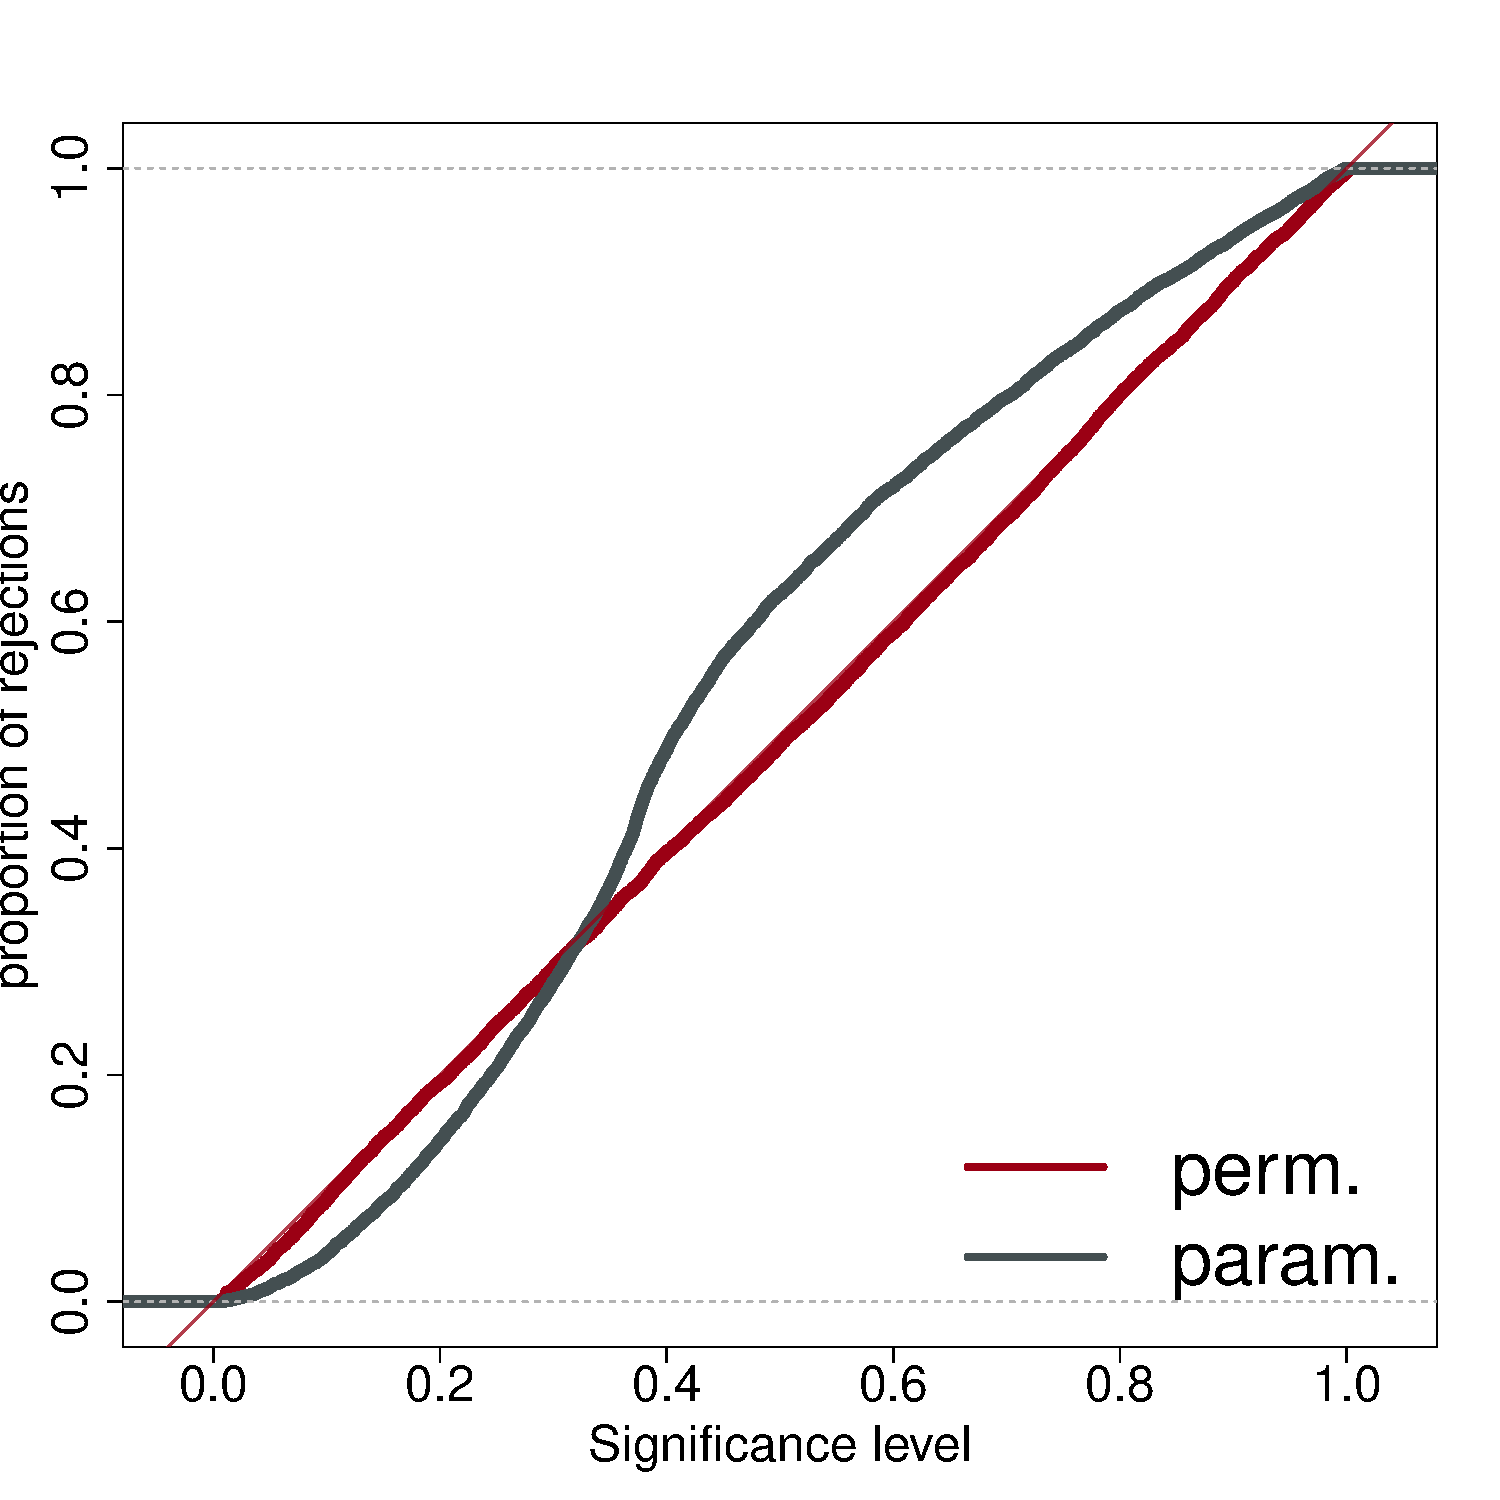
\includegraphics[width=0.55\textwidth]{figures/sim2} 
\end{center}

\begin{table}[ht]
\centering
\begin{tabular}{rrrrrr}
\hline
Empirical Type I error & $\leq$0.01 & $\leq$0.05 & $\leq$0.1 & $\leq$0.5 & $\leq$0.75 \\ 
\hline
Permutation & 0.00 & 0.04 & 0.09 & 0.49 & 0.74 \\ 
Paramatric t.test  & 0.00 & 0.01 & 0.04 & 0.62 & 0.84 \\
\hline
\end{tabular}
\end{table}
\end{frame}
%%%%%%%%%%%%%%%%%%%%%%%%%%%%%%%%
  \bfr{Simulation: $H_1$}
now $(y|grp=A)\sim Cauchy(0)$, $(y|grp=B)\sim Cauchy(10)$
  \begin{center}
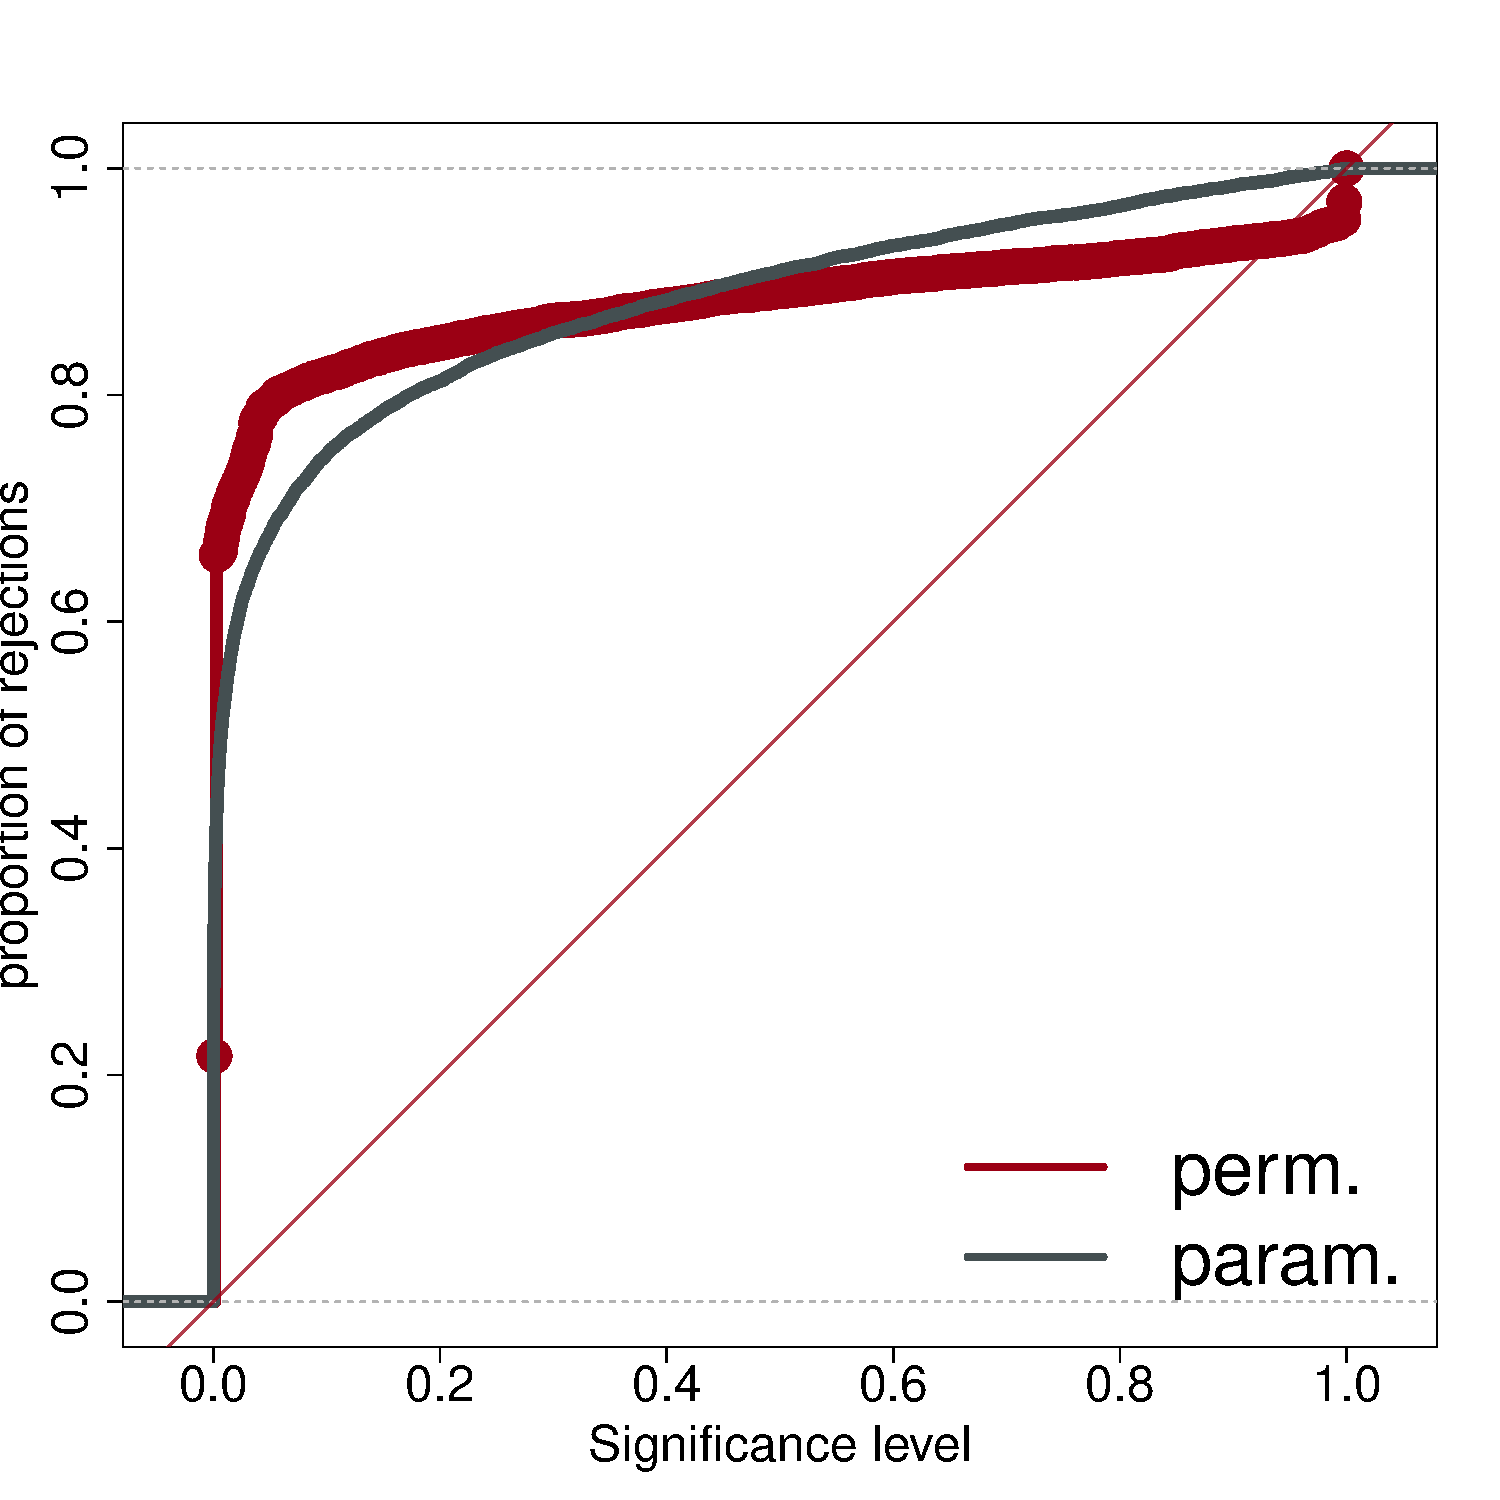
\includegraphics[width=0.55\textwidth]{figures/sim3} 
\end{center}

\begin{table}[ht]
\centering
\begin{tabular}{rrrrrr}
\hline
Empirical Power & $\leq$0.01 & $\leq$0.05 & $\leq$0.1 & $\leq$0.5 & $\leq$0.75 \\ 
\hline
Permutation & 0.66 & 0.78 & 0.81 & 0.89 & 0.92 \\ 
Paramatric t.test & 0.53 & 0.68 & 0.75 & 0.91 & 0.96 \\ 
\hline
\end{tabular}
\end{table}
\end{frame}

%%%%%%%%%%%%%%%%%%%%%%%%%%%%%%%%
%%%%%%%%%%%%%%%%%%%%%%%%%%%%%%%%
\section{Other cases}
\bfr{A very general approach}
This approach (Orbit $\Orbit$ + Test statistic $T$) is very general.\\ It includes:
\bi
\item ChiSquare test
\item Fisher exact test
\item McNemar test
\item rank tests
\item ANOVA tests
\item linear models
\item other models difficult to deal within the parametric framework
\item \ldots
\ei
\end{frame}
%%%%%%%%%%%%%%%%%%%%%%%%%%%%%%%%
\bfr{The case of contingency table}
\begin{table}[ht]
\centering
\begin{tabular}{lrrr}
  \hline
$x\setminus y$ & 0 & 1 & 2 \\ 
  \hline
A &   4 &   3 &   0 \\ 
  B &   1 &   2 &   4 \\ 
   \hline
\end{tabular}
\end{table}
{\tt > chisq.test(x,y)}\\
{\tt
  Pearson's Chi-squared test\\
data:  x and y\\
X-squared = 6, df = 2, p-value = 0.04979}

\rbf{\tt Warning message:\\
In chisq.test(x, y) : Chi-squared approximation may be incorrect}

\end{frame}

\bfr{The case of contingency table}
Use: \rbf{simulate.p.value = TRUE}\\
{\tt > chisq.test(x,y,\rbf{simulate.p.value = TRUE})\\
  Pearson's Chi-squared test (based
  on 2000 replicates)\\
data:  x and y\\
X-squared = 6, df = \rbf{NA}, p-value = 0.09345}

\bigskip
Same schema:
\bi
\item Orbit $\Orbit$: all possible permutation of $\yy$ (under $H_0$ $\xx$ and $\yy$ are independent)
\item test statistic $T(\yy^*)$: the $\chi^2$ statistic computed (higher is better)
\item p-value: proportion of $T^*$ greater than the one computed on observed data $\yy$: $p=\sum_{\yy^*\in\Orbit}I(T(\yy^*)\geq T(\yy))/|\Orbit|$.
\ei

\end{frame}

%%%%%%%%%%%%%%%%%%%%%%%%%%
\bfr{The case of experimental design with blocks \\ (or within-subject)}
For example: $n$ lots/subjects, each with two treatments (A vs B)\\
we can assume a specific effect for each lot/subject: 
$$y_{ij}\sim (\nu_i+\mu_j,\sigma_{i})\ i=1,\ldots,n,\ j=A,B$$

$$H_0: \mu_A=\mu_B \Leftrightarrow \mu_A-\mu_B=0$$

Parametric approach:
\bi
\item define:
$z_i=y_{iB}-y_{iA}\sim (\mu_B-\mu_A,2\cdot\sigma_{i})\ i=1,\ldots,n$
\item assume $\sigma_{i}=\sigma,\ \forall i=1,\ldots,n$
\item perform a 1-sample t-test (i.e. t-test for 2 paired samples)
\item test is exact only it $z_i$ is normal, it is aproximated otherwise.
\ei
\end{frame} 
%%%%%%%%%%%%%%%%%%%%%%%%%%
\bfr{The case of experimental design with blocks\\ (or within-subject)}
What about permutation approach?
how to define the Orbit $\Orbit$?

$H_0\Rightarrow \mu_A=\mu_B =\mu \Rightarrow y_{ij}\sim (\nu_i+\mu,\sigma_{i})\ i=1,\ldots,n,\ j=A,B$
\begin{eqnarray*}
&&f(\gbf{y_{1A}},\rbf{y_{1B}},\gbf{y_{2A}},\rbf{y_{2B}},\ldots,\gbf{y_{nA}},\rbf{y_{nB}}) \textrm{(observed)} =\\
&=&f(\rbf{y_{1A}},\gbf{y_{1B}},\gbf{y_{2A}},\rbf{y_{2B}},\ldots,\rbf{y_{nA}},\gbf{y_{nB}})=\\
&=&f(\gbf{y_{1A}},\rbf{y_{1B}},\rbf{y_{2A}},\gbf{y_{2B}},\ldots,\rbf{y_{nA}},\gbf{y_{nB}})\ldots
\end{eqnarray*}
\bi
\item We exchange observations only within the same lot/subject!
\item There are $2^n$ possible configurations: $|\Orbit|=2^n$
\item we don't need to assume: $\sigma_{i}=\sigma,\ \forall i=1,\ldots,n$
\item (even we may allow non addictive effect:
$\nu_{ij} \neq \nu_i+\mu_j$)
\item A part from $\Orbit$, the procedure is the same.
\ei
\end{frame} 

%%%%%%%%%%%%%%%%%%%%%%%%%%
\section{Multivariate Testing}

%%%%%%%%%%%%%%%%%%%%%%%%%%%%%%%%
\bfr{Multivarite hypotheses}
Testing $H_0(weight)$ + Testing $H_0(leaf.length)$\\
is different from testing
\bi
\item $H_0:\ H_0(weight)\ \cap \ H_0(leaf.length)$\\ (i.e. simultaneously true)
\item[] vs
\item $H_1:\ H_1(weight)\ \cup \ H_1(leaf.length)$\\
(i.e. at least one null hypo is false)
\ei
Here test $H_0$: the New is equal to the Standard in \gbf{both variables}\\
For 1-tailed alternative:\\ $p_{weight}=.098$ and $p_{leaf.length}=.030$. \\
Shall we reject the multivariate $H_0$?
\end{frame}

%%%%%%%%%%%%%%%%%%%%%%%%%%%%%%%%
\bfr{Multivariate hypotheses}
Common approaches:
\bi
\item MANOVA test 
\bi
 \item[] is OK but only for linear models (2 or more samples).
 \item[] assumes multivariate normality.
 \item[] Does not allow for one-sided alternatives.
 \ei
\item Bonferroni correction ($p=min(p_1,p_2)*2$)
\bi
\item[] very simple, always valid
\item[] does not take in account dependences among data\\ (i.e. may be very conservative, i.e. high final p-value)
\ei
\ei
\end{frame}
%%%%%%%%%%%%%%%

\bfr{Joint distributions of the data}
The two variables are dependent:
\begin{center}
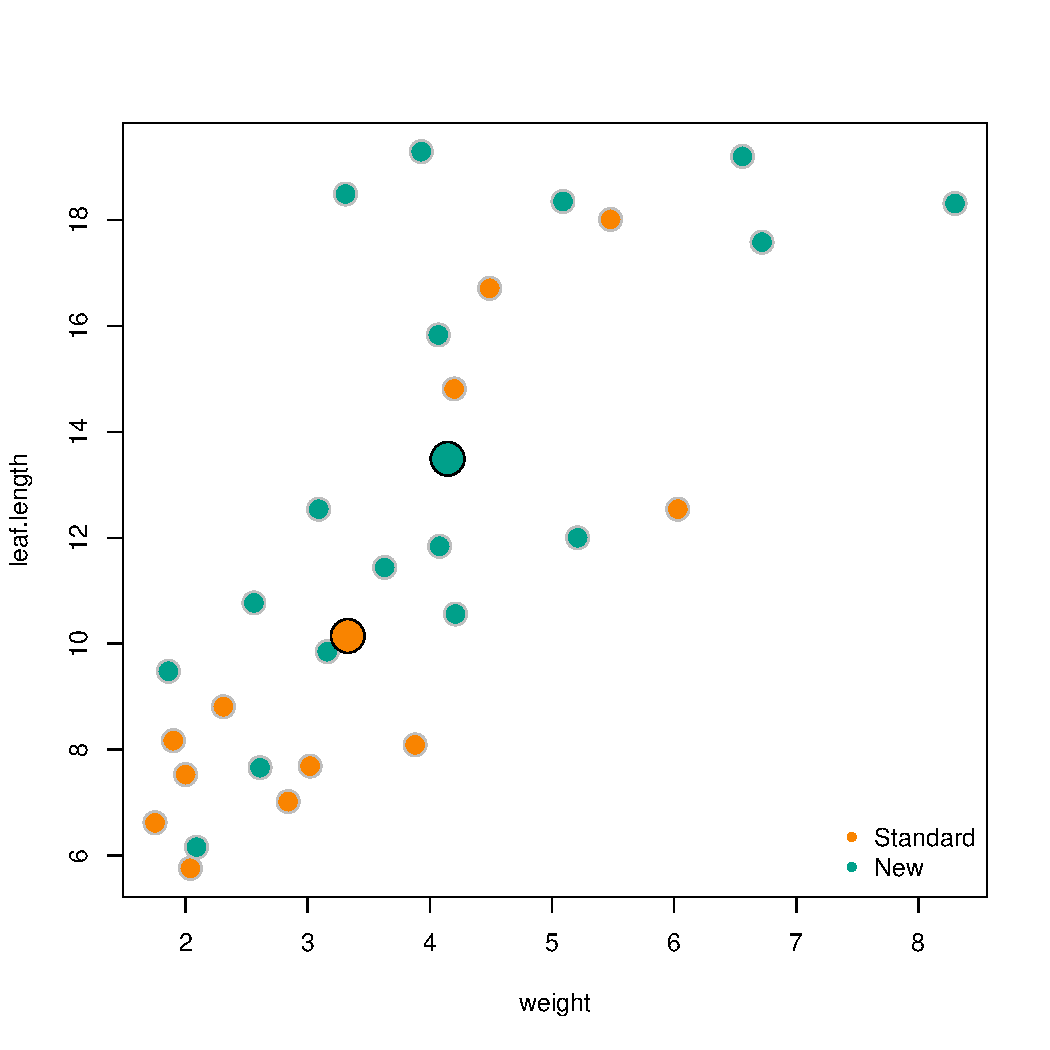
\includegraphics{figures/seeds_scatter}
\end{center}
\end{frame}
%%%%%%%%
\bfr{Joint distributions of test statistics}
This dependence induce a dependence into the joint distribution of the test statistic
\begin{center}
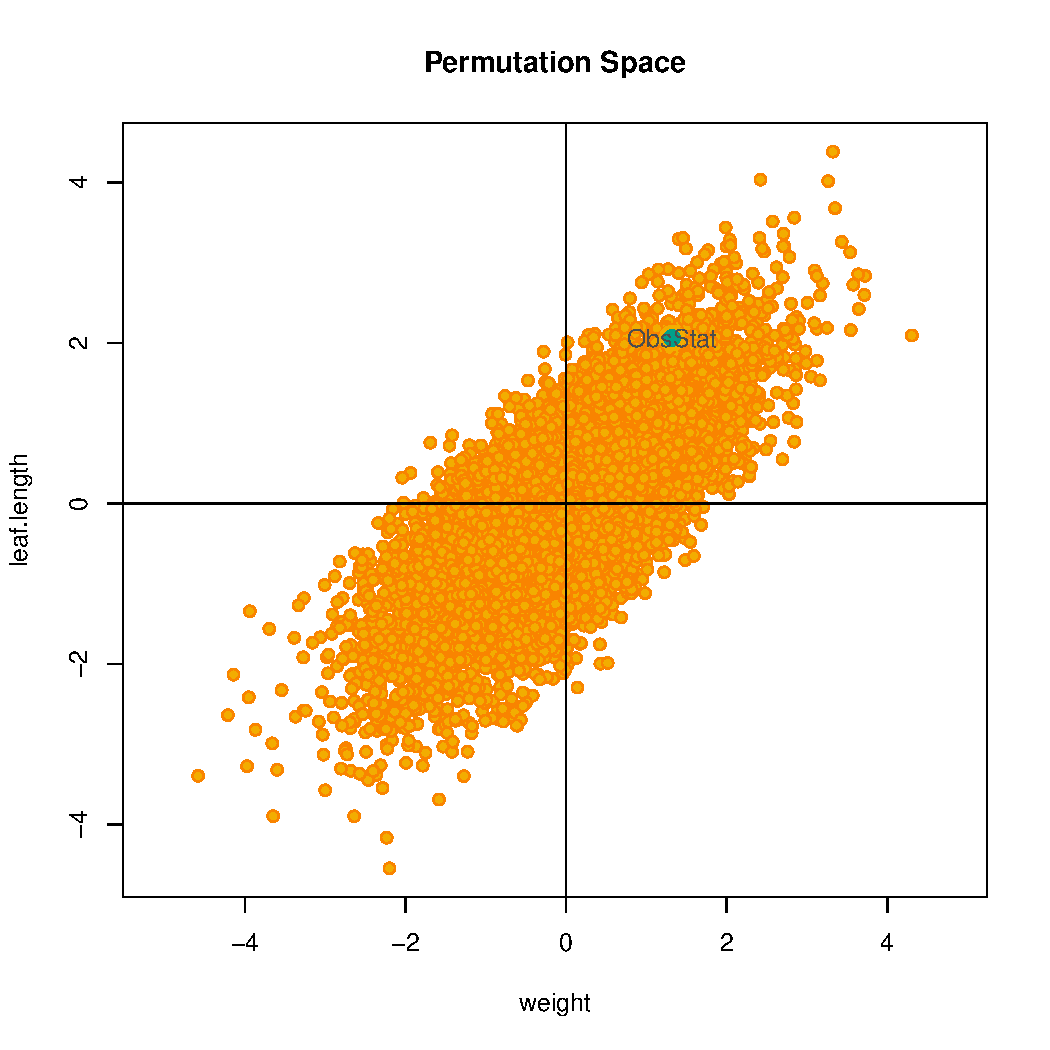
\includegraphics{figures/permT}
\end{center}
\end{frame}
%%%%%%%%5
\bfr{Joint distributions of the p-values}

... and into the p-values joint distributions
(i.e. compute the p-values for observed samples and all elements $\yy^*\in \Orbit$ )
\begin{center}
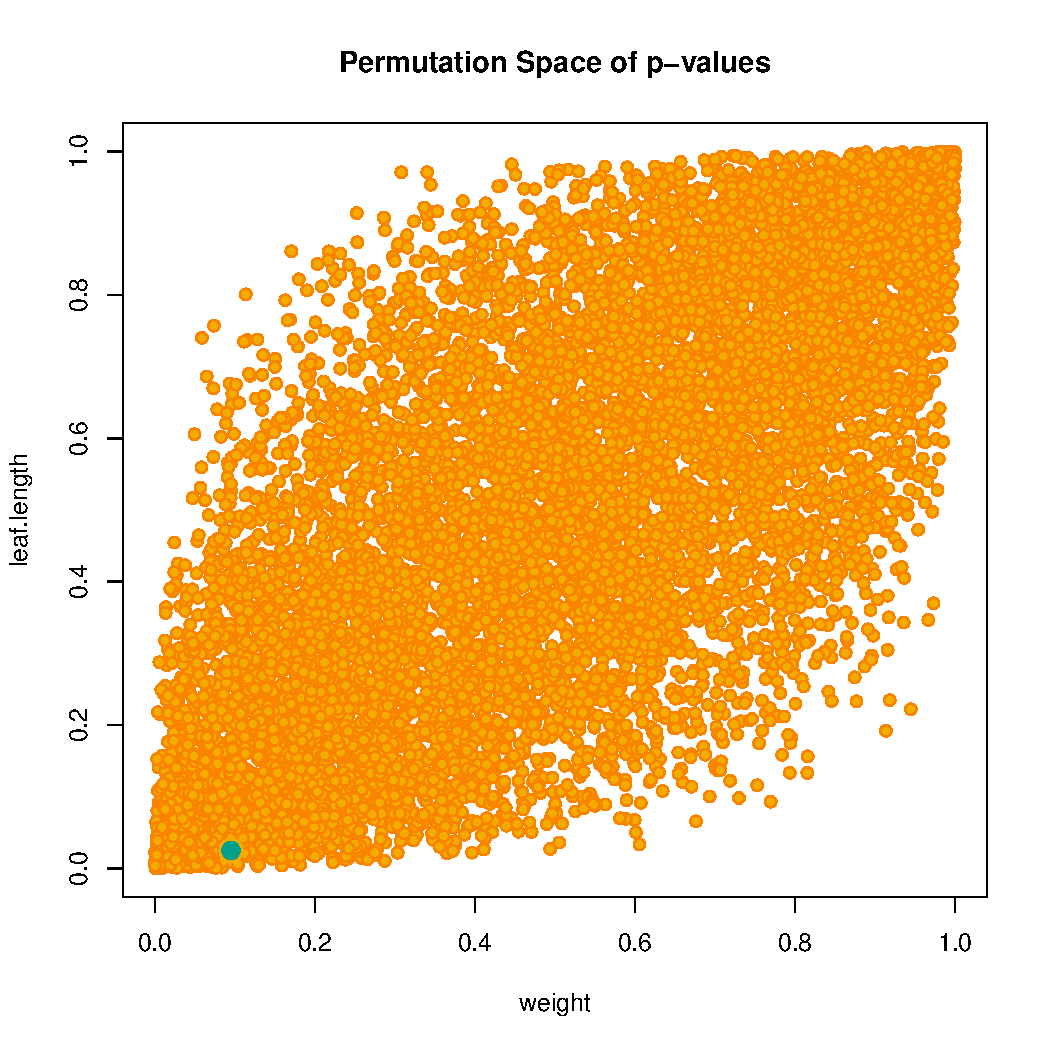
\includegraphics{figures/permP}
\end{center}
\end{frame}
%%%%%%%%%%%%%%%%%%%%%%%%%%%%%%%%
\bfr{Nonparametric Combination methodology \\
(Pesarin, 2001)}
The Orbit is now defined in a multivariate framework:
$\Orbit=\{(\yy_1,\yy_2)^*:f((\yy_1,\yy_2)^*)=f((\yy_1,\yy_2))\}$\\
(in practice: when you permute one observation in a variable, do the same in the other variables)

Also compute the $p_1^*,p_2^*$ associated to each
$\yy_1^*,\yy_2^*$.\pause

Define a Combining Function $\psi(p_1,\ldots,p_m)$ having the following properties:
\bi
\item[i] is non-increasing in each argument:
$p_k<p_k^{'}$ implies
$\psi(\ldots, p_k, \ldots) \geq \psi(\ldots,p_k^{'},\ldots)$;
\item[ii] attains its supremum $\psi^\circ$ if at least one argument attains 0;
\item[iii] $\alpha>0$ implies the critical value is such that $T_{\psi\alpha}<\psi^\circ$,
i.e. no concentration of points at $\psi^\circ$ under $H_0$.
\ei

Apply $T((p_1,p_2)^*)=\psi ((p_1,p_2)^*)$
and compute the $p_{global}$.
\end{frame}

\bfr{Fisher combining function}
$\psi = - 2\cdot (log(p_1)+log(p_2)) = 6.029$\\
$p_{global}= 0.0400$


% # calcolo il vettore dei p-values sulla base del vettore di statistiche test
% #vettore logico che individua tutti i p-value (ottenuti da permutazioni casuali) che sono <= al p-value combinato osservato
\begin{center}
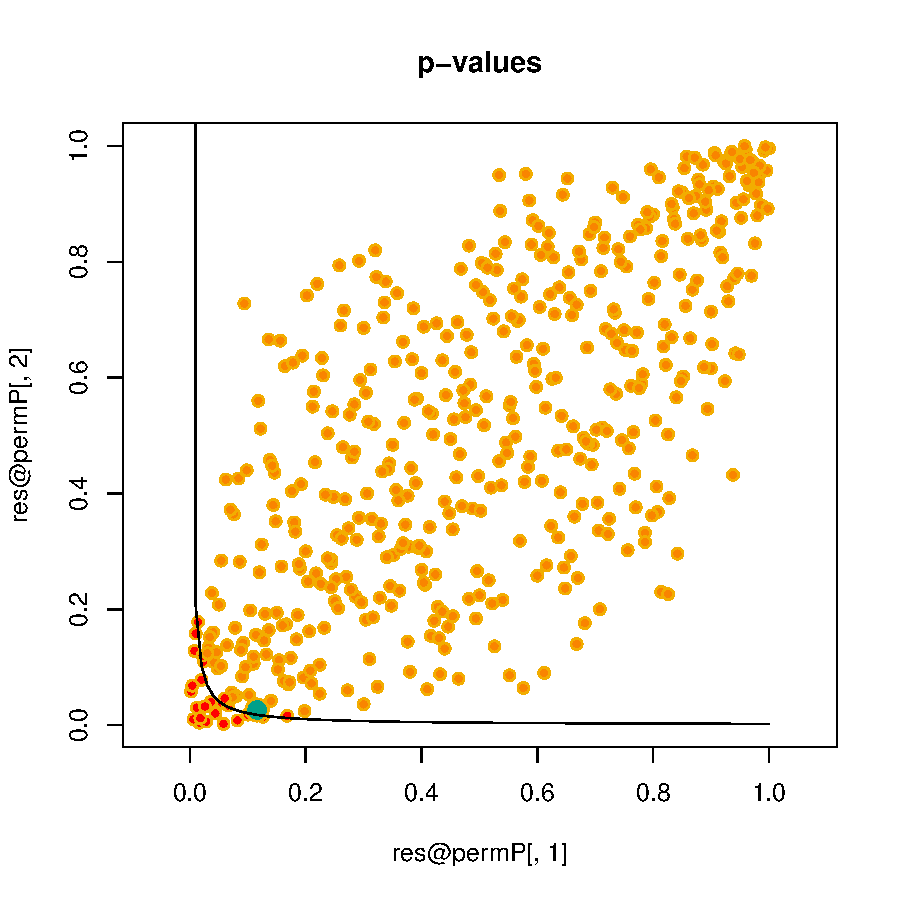
\includegraphics[width=0.7\textwidth]{figures/bivariate_temp-009}
\end{center}
% la statistica test osservata  pari a -6.19138 = -log(p-value x) -log(p-value y) 
%  ( salvato in res.fish\@permP\[1\] )
% la seguente iperbole  il luogo dei punti con la stessa statistica test:
\end{frame}

\bfr{Tippett (min-p) combining function}
$\psi =1 - min(p_1,p_2) = 1 - 0.0280$\\
$p_{global} = 0.0460$ ($\leq 2\cdot 0.0280=0.0560$ similar to Bonferroni, but more powerfull)
\begin{center}
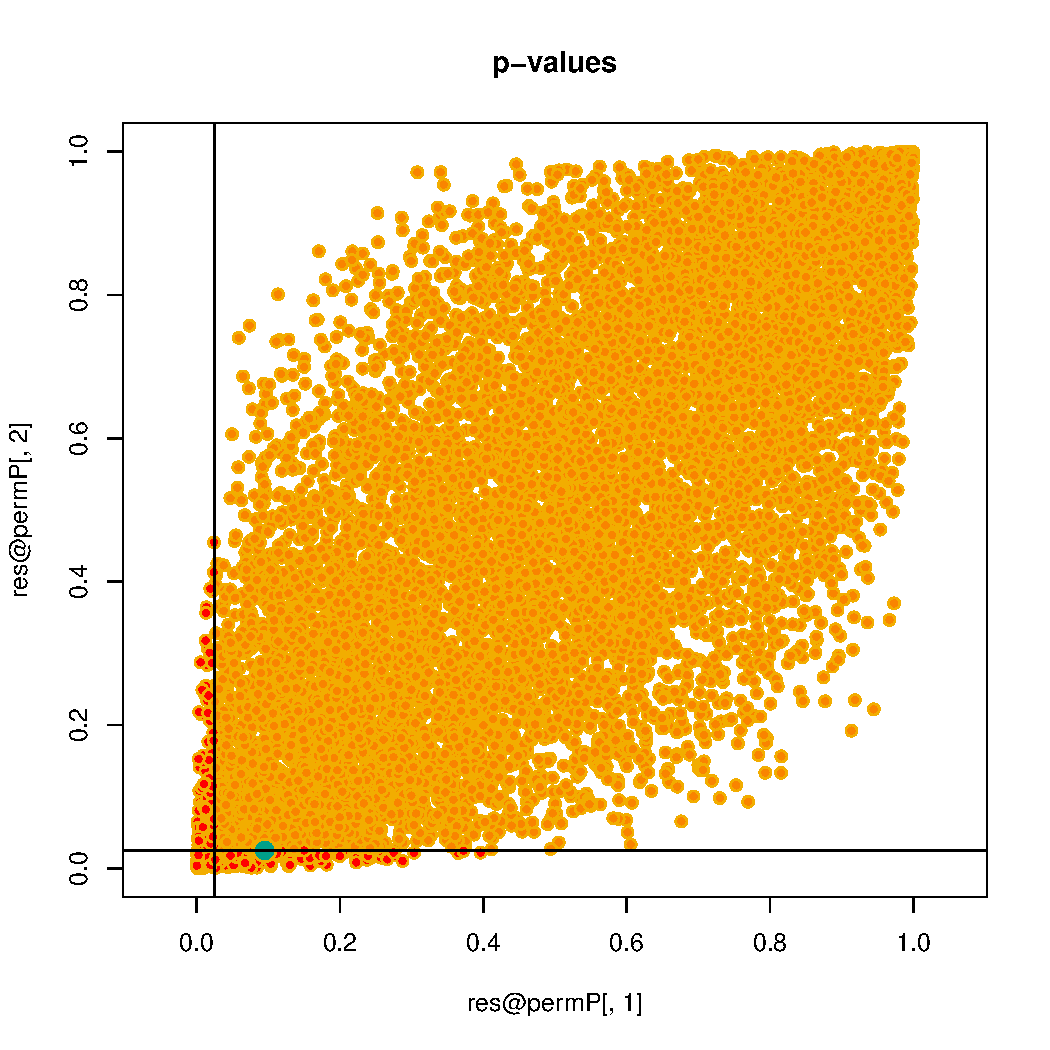
\includegraphics[width=0.7\textwidth]{figures/tippett}
\end{center}
\end{frame}
%%%%%%%%%%%%%%%%%
\bfr{Multiple testing}

\bi
\item Here we only have global p-values 
(in analogy to Manova, F-tests etc). \pause
\item If the test is significant at least one among
$H_0(weight)$ or $H_0(leaf.len)$ is false.
\item We don't know which one!
(weak control of the FamilyWise Error)\pause
\item How to cast them into multiple testing procedures? \pause
\item (strong) control of the FWER is easy!
\ei

\end{frame}
%%%%%%%%%%%%%%%%%%%%%
\begin{frame}
\frametitle{Closed Testing\footnote{R Marcus, E Peritz, KR Gabriel (1976). On closed testing procedures with special reference to ordered analysis of variance. Biometrika 63: 655-660.}}

Test in each node: any multivariate permutation test\\
(eg alternative to Manova)

\begin{center}
\bbf{Closure Set}

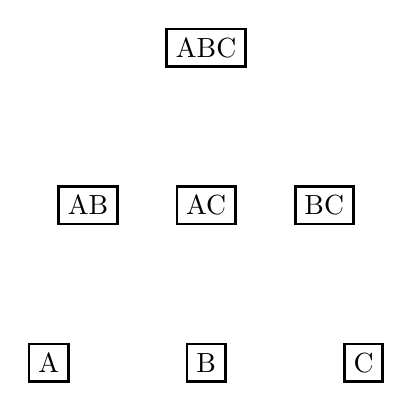
\begin{tikzpicture}
\draw[] 
(0,4) node[draw, line width=1pt] {ABC}
(-1.5,2) node[draw, line width=1pt] {AB}
(0,2) node[draw, line width=1pt] {AC}
(1.5,2) node[draw, line width=1pt] {BC}
(-2,0) node[draw, line width=1pt] {A}
(0,0) node[draw, line width=1pt] {B}
(2,0) node[draw, line width=1pt] {C};
\end{tikzpicture}
\end{center}

Adjusted $\tilde p_A=\max(p_A,p_{AB},p_{AC},p_{ABC})$

\end{frame} 
%%%%%%%%%%%%%%%%%%%%%
\begin{frame}
\frametitle{Westfall \& Young min-p (and max-t) \footnote{
Resampling-based multiple testing: Examples and methods for p-value
adjustment, volume 279. Wiley-Interscience, 1993.}}

Close testing infeasible when with many hypos ($2^m-1$ tests).

Westfall \& Young min-p: shortcut using min-p combining function ($m$ tests).
\pause

Suppose three hypotheses tested and $p_A\leq p_B \leq p_C$

\bi
  \item Test $H_A$, $H_B$ and $H_C$ using min-p: $p_{ABC}$
    \bi 
      \item if $p_{ABC}\leq\alpha$ reject $H_A$ and go on
      \item if $p_{ABC}>\alpha$ STOP
    \ei
  \item Test $H_B$ and $H_C$ using min-p: $p_{BC}$
    \bi 
      \item if $p_{BC}\leq\alpha$ reject $H_B$ and go on
      \item if $p_{BC}>\alpha$ STOP
    \ei
  \item Test $H_C$: $p_{C}$
    \bi 
      \item if $p_{C}\leq\alpha$ reject $H_C$ and STOP
      \item if $p_{C}>\alpha$ STOP
    \ei
\ei

For max-t procedure substitute $p_{ABC}\leq\alpha$  with $t_{ABC}\geq t_\alpha$

\end{frame} 

%%%%%%%%%%%%%%%%%
\bfr{Take Home Message}
Permutation approach:
\bi
\item very general uni/multi-variate approach
\item few assumptions on the data-generating process
\item natural approach in {\bf  randomized experimental design}
\item good inferential properties\\ (in most of the cases: exact control of the type I error, consistency, asymptotic optimality)
\item very convenient for multiplicity control methods, since it deals easily with dependent tests.
\ei
Warnings:
\bi
\item more complex experimental design can be dealt, but with caution (Pesarin, 2001) 
\item multiple (generalized) linear models need some care\\ (Solari, Finos \& Goeman, 2014 and other work in progress)
\ei
Software `R`: libraries `coin`,`flip`: `flip(); flip.adjust()`
\end{frame}
%%%%%%%%%%%%%%%%%
\end{document}
